% \newgeometry{top=4cm,left=4cm,right=4cm,bottom=4cm} 
%
\section{Two-point functions of chiral primary operators}\label{sec:CPO}
In the following section we concern ourselves with the computations of two-point functions between a certain type of local single-trace scalar operators in $\mathcal{N} = 4$ SYM; namely oprators of the following simple form.
%
%
\begin{equation}\label{chiral_primaries}
\mathcal{O}_{\boldsymbol{Z}} = \tr \boldsymbol{Z}^L
%
\quad , \quad
%
\mathcal{O}_{\boldsymbol{X}} = \tr \boldsymbol{X}^L
%
\quad , \quad
%
\boldsymbol{Z} = \boldsymbol{\phi}_3 + i \, \boldsymbol{\phi}_6
%
\quad , \quad
%
\boldsymbol{X} = \boldsymbol{\phi}_1 + i \, \boldsymbol{\phi}_4
\end{equation}
%
%
Where we have suppressed the spacetime dependence of all scalar fields in the above definitions, to avoid notational clutter. We will attempt to compute two-point functions between the above operators using the standard field theoretic perturbative technique of Feynman diagrams, which is only possible due to the ground work layed out in section \ref{sec:dCFT} (\textit{gauge fixing, mass matrix diagonalization etc.}). The reason we focus on these operators in particular is very pratical; the local operators $\mathcal{O}_{\boldsymbol{Z}}$ and $\mathcal{O}_{\boldsymbol{X}}$ are perhaps some of the simplest examples of \textit{chiral primary operators}. In order to understand what makes chiral primary operators comparatively easier to study, we first have to know what they are exactly.

\subsection{Chiral primary operators in SCFTs}
In the context of super conformal field theories, a chiral primary operator is first of all a \textit{super conformal primary} operator. By definition, super conformal primary operators have to satisfy the conditions.
%
%
\begin{equation}\label{super_conformal_primary_condition}
[D, \mathcal{O}(0)] = -i \Delta \, \mathcal{O}(0)
%
\quad , \quad
%
[S^a_\alpha, \mathcal{O}(0)] = 0
%
\quad , \quad
%
[\bar{S}_{a \dot{\alpha}}, \mathcal{O}(0)] = 0
\end{equation}
%
%
Where $S^a_\alpha$ are super-partners to the generators of special conformal transformations $K_\mu$, and $D$ is the generator of dilatations (\textit{scale transformations}). Furthermore, a chiral primary operator needs to be anihilated by at least one of the super-partners $Q^a_{\alpha}$ to the generators of spacetime translations $P_\mu$.
%
%
\begin{equation}\label{chiral_primary_condition}
\exists a \in \{1,\ldots,\mathcal{N} \} \, \exists \alpha \in \{1,2 \}: \;
[Q^a_\alpha, \mathcal{O}(0)] = 0
\end{equation}
%
%
The conditions (\ref{super_conformal_primary_condition}) and (\ref{chiral_primary_condition}) together leads to a very powerful restriction on the conformal dimensions $\Delta$ of chiral primaries; namely that they can not depend on the coupling constant $g$. To show that this is indeed the case, we need the following anti-commutation relation from the super conformal algebra $\mathfrak{psu}(2,2 | 4)$ \cite{Integrability Review}.
%
%
\begin{equation}\label{super conformal algebra 1}
\{ Q^a_\alpha, S_{b\beta} \}
=
-\frac{i}{2} \, \varepsilon_{\alpha \beta} {(\sigma^{IJ})^a}_b \, R_{IJ}
- \frac{1}{2} \varepsilon_{\alpha \beta} {\delta^a}_b D
+ (\sigma^{\mu \nu})_{\alpha \beta} {\delta^a}_b \, M_{\mu \nu}
\end{equation}
%
%
Where $ {(\sigma^{IJ})^a}_b$ are the sigma matrices of the $SU(4)$ fundamental representation, $R_{IJ}$ are the generators of the $SO(6)$ R-symmetry, and $M_{\mu \nu}$ are the generators of $SO(3,1)$. If we now assume that $\mathcal{O}$ is a scalar operator, such that $[M_{\mu \nu}, \mathcal{O}(0)] = 0$, we can use the above anti-commutation relations of the super conformal algebra, the graded Jacobi identity and the aforementioned two conditions (\ref{super_conformal_primary_condition}) and (\ref{chiral_primary_condition}) to obtain.
%
%
\begin{equation*}
[\{ Q^a_\alpha, S_{b\beta} \}, \mathcal{O}(0)]
=
[
-i \, \varepsilon_{\alpha \beta} {(\sigma^{IJ})^a}_b \, R_{IJ}
- \varepsilon_{\alpha \beta} {\delta^a}_b D
,
\mathcal{O}(0)
]
=
0
\end{equation*}
%
%
\begin{equation}\label{chiral_primary_relation}
\Leftrightarrow \quad
%
{(\sigma^{IJ})^a}_b \, [R_{IJ}, \mathcal{O}(0)]
=
\Delta \, {\delta^a}_b \, \mathcal{O}(0)
\end{equation}
%
%
We have now shown that any chiral primary $\mathcal{O}$ has to satisfy (\ref{chiral_primary_relation}). It is also true that any super conformal primary $\mathcal{O}$ satisfying (\ref{chiral_primary_relation}) has to be a chiral primary. This is because.
%
%
\begin{equation}
[[ \mathcal{O}(0) , Q^a_\alpha ], S_{b\beta}] = 0
%
\quad \Rightarrow \quad
%
[ \mathcal{O}(0) , Q^a_\alpha ] = 0
\end{equation}
%
%
Since $Q^a_\alpha$ would otherwise increase the conformal dimension of $\mathcal{O}$ by $1/2$, making $S_{b\beta}$ unable to anihilate $\mathcal{O}$. Now, because the eigenvalues of the $SO(6)$ generators (\textit{also know as the R-charges}) are discrete and unchanged when interactions are included, the conformal dimensions $\Delta$ of the chiral primaries will also remain unchanged because of (\ref{chiral_primary_relation}). Thus, the conformal dimensions of chiral primaries can not receive any quantum corrections (\textit{also known as anomolus dimensions}) when interactions are included. Comming back to equation (\ref{chiral_primary_relation}), it can easily be checked using the explicit form of the ${(\sigma^{IJ})^a}_b$ matrices.
%
%
\begin{equation*}
\sigma^{14} = \text{diag}(1,1,-1,-1)
%
\quad , \quad
%
\sigma^{25} = \text{diag}(1,-1,1,-1)
%
\quad ,
\end{equation*}
%
%
\begin{equation}\label{sigmas_SU(4)}
\sigma^{36} = \text{diag}(1,-1,-1,1)
\end{equation}
%
%
That a solution to this equation is given by operators with R-charges $(J_1,0,0)$ and conformal dimension $\Delta = J_1$, for $a=1,2$. The R-charges correspond to eigenvalues of $R_{14}$, $R_{25}$ and $R_{36}$, such that.
%
%
\begin{equation}
[R_{14}, \mathcal{O}(0)] = J_1 \, \mathcal{O}(0)
%
\quad , \quad
%
[R_{25}, \mathcal{O}(0)] = [R_{36}, \mathcal{O}(0)] = 0
\end{equation}
%
%
It turns out that conformal primary operators with R-charges $(J_1,0,0)$ and $\Delta = J_1$, are also anihilated by the super-charges $\bar{Q}_{3,\dot{\alpha}}$ and $\bar{Q}_{4,\dot{\alpha}}$. This follows from yet another anti-commutation relation from the super conformal algebra $\mathfrak{psu}(2,2|4)$, together with (\ref{sigmas_SU(4)}).

\newpage
%
%
\begin{equation}\label{super conformal algebra 2}
\{ \bar{Q}_{a \dot{\alpha}}, \bar{S}^b_{\dot{\beta}} \}
=
\frac{i}{2} \, \varepsilon_{\dot{\alpha} \dot{\beta}} {(\sigma^{IJ})_a}^b \, R_{IJ}
- \frac{1}{2} \varepsilon_{\dot{\alpha} \dot{\beta}} {\delta_a}^b D
+ (\sigma^{\mu \nu})_{\dot{\alpha} \dot{\beta}} {\delta_a}^b \, M_{\mu \nu}
\end{equation}
%
%
\begin{equation}
\quad \Leftrightarrow \quad
%
{(\sigma^{IJ})_a}^b \, [R_{IJ}, \mathcal{O}(0)]
=
-\Delta \, {\delta_a}^b \, \mathcal{O}(0)
\end{equation}
%
%
Thus, the operators with R-charges $(J_1,0,0)$ and $\Delta = J_1$ are anihilated by half of the translational super charges. Such operators are referred to as \textit{$1/2$-BPS operators}. Of cause there is nothing particularly special about the R-charges $(J_1,0,0)$, compared to the $(0,J_2,0)$ or the $(0,0,J_3)$ R-charges. Therefore, operators which have these collections of R-charges also solve (\ref{chiral_primary_relation}) for half the values of $a$ and $\dot{\alpha}$, given that $\Delta$ is chosen analogously. Now that we know that these types of operators constitute chiral primaries, we can quickly verify that $\mathcal{O}_{\boldsymbol{Z}}$ and $\mathcal{O}_{\boldsymbol{X}}$ are indeed such operators. With the definitions of ${\boldsymbol{X}}$ and ${\boldsymbol{Z}}$ given in (\ref{chiral_primaries}), it is easy to verify that.
%
%
\begin{equation}
[R^{(0)}_{14}, \mathcal{O}_{\boldsymbol{X}}(0)] = L \, \mathcal{O}_{\boldsymbol{X}}(0)
%
\quad , \quad
%
[R^{(0)}_{36}, \mathcal{O}_{\boldsymbol{Z}}(0)] = L \, \mathcal{O}_{\boldsymbol{Z}}(0)
\end{equation}
%
%
\begin{equation}
[D^{(0)}, \mathcal{O}_{\boldsymbol{X}}(0)] = -i \, L \, \mathcal{O}_{\boldsymbol{X}}(0)
%
\quad , \quad
%
[D^{(0)}, \mathcal{O}_{\boldsymbol{Z}}(0)] = -i \, L \, \mathcal{O}_{\boldsymbol{Z}}(0)
\end{equation}
%
%
Where $D^{(0)}$ and $R^{(0)}_{IJ}$ denotes the dilatation operator and $SO(6)$ generators respectively, at zero coupling. Thus, we see that for the free theory, these operators have the R-charges $(L,0,0)$ and $(0,0,L)$, and conformal dimensions $\Delta = J_1 = L$ and $\Delta = J_3 = L$ respectively. Furthermore, since $\mathcal{O}_{\boldsymbol{Z}}$, $\mathcal{O}_{\boldsymbol{X}}$ are constructed out of scalar fields only, and the scalar fields have the lowest conformal dimension of all $\mathcal{N}=4$ fields, they must indeed be super conformal primaries. Because $\mathcal{O}_{\boldsymbol{X}}$ and $\mathcal{O}_{\boldsymbol{Z}}$ are super conformal primaries, and also solve the equation (\ref{chiral_primary_relation}) at zero coupling, they must also commute with half the translational supercharges at zero coupling. Because the number of operators in a given $\mathfrak{psu}(2,2|4)$ representation does not depend on the coupling, we conclude that the operators $\mathcal{O}_{\boldsymbol{X}}$ and $\mathcal{O}_{\boldsymbol{Z}}$ have R-charges $(L,0,0)$ and $(0,0,L)$, and conformal dimensions $\Delta = L$, for all values of the coupling constant $g$.\\
Instead of thinking of chiral primaries as operators with a given set of R-charges, it is often useful to think of them as elements of some tensor representation of $SU(4) \simeq SO(6)$. The operators $\mathcal{O}_{\boldsymbol{X}}$ and $\mathcal{O}_{\boldsymbol{Z}}$ in particular turn out to be highest weight operators of the $L$-fold symmetric-traceless representation of $SO(6)$.
%
%
\begin{equation}
\mathcal{O}_{\boldsymbol{X}}
=
\Phi_{\boldsymbol{X}}^{i_1 \ldots i_L}
\tr[
\boldsymbol{\phi}_{i_1} \cdots \boldsymbol{\phi}_{i_L}
]
%
\quad , \quad
%
\mathcal{O}_{\boldsymbol{Z}}
=
\Phi_{\boldsymbol{Z}}^{i_1 \ldots i_L}
\tr[
\boldsymbol{\phi}_{i_1} \cdots \boldsymbol{\phi}_{i_L}
]
\end{equation}
%
%
Where the wavefunctions $\Phi_{\boldsymbol{X}}^{i_1 \ldots i_L}$ and $\Phi_{\boldsymbol{Z}}^{i_1 \ldots i_L}$, are symmetric and traceless in any pair of indices. To see that this is indeed the case, let us look at $\mathcal{O}_{\boldsymbol{Z}}$ as an example. Expanding ${\boldsymbol{Z}}$-field number $\ell$ and $\ell+1$ in the trace, we find that.

\newpage
%
%
\begin{equation*}
\cdots
{\boldsymbol{Z}}
(\boldsymbol{\phi}_3 + i \boldsymbol{\phi}_6) (\boldsymbol{\phi}_3 + i \boldsymbol{\phi}_6)
{\boldsymbol{Z}}
\cdots
\end{equation*}
%
%
\begin{equation}
=
\cdots
{\boldsymbol{Z}}
(
\boldsymbol{\phi}_3 \boldsymbol{\phi}_3 - \boldsymbol{\phi}_6 \boldsymbol{\phi}_6
+ i \boldsymbol{\phi}_3 \boldsymbol{\phi}_6 + i \boldsymbol{\phi}_6 \boldsymbol{\phi}_3
)
{\boldsymbol{Z}}
\cdots
\end{equation}
%
%

%
%
\begin{equation*}
\Phi_{\boldsymbol{Z}}^{\ldots 36 \ldots} = \Phi_{\boldsymbol{Z}}^{\ldots 63 \ldots}
%
\quad , \quad
%
\Phi_{\boldsymbol{Z}}^{\ldots 33 \ldots} + \Phi_{\boldsymbol{Z}}^{\ldots 66 \ldots} = 0
%
\quad ,
\end{equation*}
%
%
\begin{equation}\label{Phi_Z_properties}
\Phi_{\boldsymbol{Z}}^{\ldots i_\ell i_{\ell+1} \ldots} = 0
%
\quad \text{for} \quad
%
i_\ell, i_{\ell+1} \neq 3,6
\end{equation}
%
%
Using the information contained in (\ref{Phi_Z_properties}), we can now conclude that the wavefunction $\Phi_{\boldsymbol{Z}}^{i_1 \ldots i_L}$ obeys.
%
%
\begin{equation}
\Phi_{\boldsymbol{Z}}^{i_1 \ldots i_{\ell} \, i_{\ell+1} \ldots i_L}
=
\Phi_{\boldsymbol{Z}}^{i_1 \ldots i_{\ell+1} i_{\ell} \ldots i_L}
% have already seen
\quad , \quad
%
\sum_{i_{\ell}=1}^6
\Phi_{\boldsymbol{Z}}^{i_1 \ldots i_{\ell} \, i_{\ell} \ldots i_L}
=
0
\end{equation}
%
%
It is clear that by the same arguments, the wavefunction $\Phi_{\boldsymbol{X}}^{i_1 \ldots i_L}$ also has exactly the above properties.

\subsection{Symmetries and the form of two-point functions in dCFTs}\label{form of two-point functions in dCFT}
Before we make any attempts to compute the leading order corrections to any two-point functions, let us briefly discuss how the remaining unbroken symmetries in our dCFT setups restrict the forms of scalar two-point functions. Firstly, the unbroken $SO(2,1)$ Poincar\'e invariance parallel to the defect, dictates that any scalar two-point function $\expval{\mathcal{O}_a(x) \mathcal{O}_b(y)}$ must be a function of the combination $|\vec{x} - \vec{y}|$. Here, $x$, $y$ are any points on the $x_3,y_3 > 0$ side of the defect, and $|\vec{x} - \vec{y}|$ is the standard Euclidian norm. We additionally use the notation. 
%
%
\begin{equation}
x = (\vec{x}, x_3)
%
\quad , \quad
%
\vec{x} = (x_0, x_1, x_2)
%
\quad , \quad
%
|x-y|^2 = |\vec{x} -\vec{y}|^2 + |x_3 - y_3|^2
\end{equation}
%
%
We can further restrict the form of $\expval{\mathcal{O}_a(x) \mathcal{O}_b(y)}$ by taking advantage of the fact that the discrete symmetry known as \textit{inversion}, also remains unbroken by the non-zero vevs.
%
%
\begin{equation}\label{inversion}
x \to \tilde{x} = \frac{x}{|x|^2}
%
\quad \Rightarrow \quad
%
|x| \to |\tilde{x}| = \frac{|x|}{|x|^2} = \frac{1}{|x|}
%
\quad \Rightarrow \quad
%
\tilde{x} \to \frac{\tilde{x}}{|\tilde{x}|^2}
=
x
\end{equation}
%
%
The invariance under inversion and $SO(2,1)$ Poincar\'e symmetries greatly restricts the possible forms of $\expval{\mathcal{O}_a(x) \mathcal{O}_b(y)}$, which stems from the fact that only one so called \textit{conformal ratio} $\xi$, can be constructed such as to be invaraint under the aforementioned symmetries. Using (\ref{inversion}) we find that.
%
%
\begin{equation}\label{conformal_ratios}
|\tilde{x}-\tilde{y}|^2 = \frac{|x-y|^2}{x^2 y^2}
%
\quad , \quad
%
\tilde{x}_3 \tilde{y}_3 =\frac{x_3 y_3}{x^2 y^2}
%
\quad , \quad
%
\xi = \frac{|x-y|^2}{4 x_3 y_3}
%
\quad \Rightarrow \quad
%
\tilde{\xi} = \xi
\end{equation}
%
%
Finally, to ensure the correct scaling under the last unbroken symmetry: $SO(1,1)$ \textit{scale transformations}, the two-point functions are forced to be of the following form. 
%
%
\begin{equation}
x \to \tilde{x} = \lambda x
%
\quad , \quad
%
\mathcal{O}_a(x) \to \tilde{\mathcal{O}}_a(x)
=
\lambda^{-\Delta_a} \mathcal{O}_a(\lambda^{-1} x)
\end{equation}
%
%
\begin{equation}
\Rightarrow \quad
%
\expval{\mathcal{O}_a(x) \mathcal{O}_b(y)}
=
\frac{f_{ab}(\xi)}{(2 x_3)^{\Delta_a} (2 y_3)^{\Delta_b}}
\end{equation}
%
%
We now see that the only freedom left on the form of scalar two-point functions are encoded in the functions $f_{ab}(\xi)$, which depend only on the scalar operators in question and the conformal ratio $\xi$. Thus, for chiral primary operators, which have their conformal dimension $\Delta$ protected, the information that we want to later extract from our perturbative computations are exactly these conformal functions $f_{ab}(\xi)$.\\
Another way to extract information about two-point functions based on symmetry is to consider the limit of points far away from the defect. We know that the scalar vevs vanish when we take the distance from the defect to $\infty$, which means that the two-point function should reduce to the standard form dictated by the full $SO(4,2)$ symmetry.
%
%
\begin{equation}
\lim_{z_3 \to \infty} \expval{\mathcal{O}_a(x+z) \bar{\mathcal{O}}_b(y+z)}
=
\frac{M_{ab}}{|x-y|^{\Delta_a + \Delta_b}}
\end{equation}
%
%
From this consideration we learn two things. Firstly, we see that conformal dimensions of operators remain unchanged in this limit. Therefore, if we want to find corrections to the conformal dimensions of operators caused by interactions, it will be easier to do the analysis in the standard $\mathcal{N}=4$ theory and subsequently carry over the results to the defect theory. More on how to do this in section \ref{sec:NPO}. Secondly, to ensure the correct limiting behavior of the conformal functions $f_{ab}(\xi)$ when going far from the defect, they must be of the following form.
%
%
\begin{equation}
f_{ab}(\xi) = \xi^{-\frac{\Delta_a + \Delta_b}{2}} \left[
M_{ab} + \sum_{n=1}^\infty c_{ab,n} \, \xi^n
\right]
\end{equation}
%
%
Thus, we can not have terms with arbitrarily high negative powers of $\xi$ appearing in the conformal functions $f_{ab}(\xi)$. This fact can provide a nice check of the results obtained by perturbative methods.

\subsection{Two-point functions at tree level (\textit{disconnected})}
In this subsection, we finally begin the computation of two-point functions between the chiral primary operators $\mathcal{O}_{\boldsymbol{X}}(x)$ and $\mathcal{O}_{\boldsymbol{Z}}(x)$. There are three different kinds of two-point functions we can make from these operators.
%
%
\begin{equation}\label{the two-point functions}
\expval{\mathcal{O}_{\boldsymbol{Z}}(x) \, \mathcal{O}_{\boldsymbol{Z}}(y)}
%
\quad , \quad
%
\expval{\mathcal{O}_{\boldsymbol{Z}}(x) \, \mathcal{O}_{\boldsymbol{\bar{Z}}}(y)}
%
\quad , \quad
%
\expval{\mathcal{O}_{\boldsymbol{X}}(x) \, \mathcal{O}_{\boldsymbol{Z}}(y)}
\end{equation}
%
%
To start of, we want to find the disconnected tree-level contribution to these two-point functions, obtained by inserting the classical values of the ${\boldsymbol{Z}}$ and ${\boldsymbol{X}}$ fields into the operators $\mathcal{O}_{\boldsymbol{X}}(x)$ and $\mathcal{O}_{\boldsymbol{Z}}(x)$.
%
%
\begin{equation*}
\expval{\tr \boldsymbol{Z}^{L_1} \tr \boldsymbol{Z}^{L_2} }_{\mathrm{tree, dc.}}
%
=
%
\tr \mathcal{Z}^{L_1}
\tr \mathcal{Z}^{L_2}
%
\quad , \quad
%
\big\langle \tr \boldsymbol{Z}^{L_1} \tr \boldsymbol{\bar{Z}}^{L_2} \big\rangle_{\mathrm{tree, dc.}}
%
=
%
\tr \mathcal{Z}^{L_1}
\tr \bar{\mathcal{Z}}^{L_2}
%
\quad ,
\end{equation*}
%
%
\begin{equation}\label{tree-level dc.}
\expval{\tr \boldsymbol{X}^{L_1} \tr \boldsymbol{Z}^{L_2} }_{\mathrm{tree, dc.}}
%
=
%
\tr \mathcal{X}^{L_1}
\tr \mathcal{Z}^{L_2}
%
\quad , \quad
%
{\boldsymbol{Z}} = \mathcal{Z} + Z
%
\quad , \quad
%
{\boldsymbol{X}} = \mathcal{X} + X
\end{equation}
%
%
Where ${\boldsymbol{\bar{Z}}}$ is simply the adjoint of ${\boldsymbol{Z}}$. Also, the spacetime dependence of the ${\boldsymbol{X}}$ and ${\boldsymbol{Z}}$ fields in the above have been suppressed to avoid notational clutter. We will continue to do so throughout this section.\\

\subsubsection[$SO(3) \times SO(3)$ symmetric vevs]{$\mathbf{SO(3) \times SO(3)}$ symmetric vevs}
The classical parts of the ${\boldsymbol{X}}$ and ${\boldsymbol{Z}}$ fields in the $\mathfrak{so}(3) \times \mathfrak{so}(3)$ symmetric setup, can easily be expressed in terms of the classical parts of the scalar fields they are constructed from (\ref{chiral_primaries}). The results are as follow.
%
%
\begin{equation}
\mathcal{Z} = \Phi_3 + i \, \Phi_6
= -\frac{1}{x^3}
\left(
t_3^{k_1} \otimes \mathbb{1}_{k_2} \oplus 0_{N-k_1 k_2}
+ i \, \mathbb{1}_{k_1} \otimes t_3^{k_2} \oplus 0_{N-k_1 k_2}
\right)
\end{equation}
%
%
\begin{equation}
\mathcal{X} = \Phi_1 + i \, \Phi_4
= -\frac{1}{x^3}
\left(
t_1^{k_1} \otimes \mathbb{1}_{k_2} \oplus 0_{N-k_1 k_2}
+ i \, \mathbb{1}_{k_1} \otimes t_1^{k_2} \oplus 0_{N-k_1 k_2}
\right)
\end{equation}
%
%
To find the tree-level contributions to (\ref{the two-point functions}), we need to evaluate $\tr \mathcal{X}^L$ and $\tr \mathcal{Z}^L$, as can be seen in (\ref{tree-level dc.}). As one might intuitively expect, there exists a unitary transformation $U$, which takes $t_1 \to t_3$ and $t_3 \to t_1$, which means that the two kinds of traces are equal.
%
%
\begin{equation}
U t_1 U^\dagger = t_3
%
\quad , \quad
%
U t_2 U^\dagger = -t_2
%
\quad , \quad
%
U t_3 U^\dagger = t_1
%
\quad , \quad
%
U = e^{i \pi t_3} e^{i \pi t_2 / 2}
\end{equation}
%
%

%
%
\begin{equation*}
\tr[ \mathcal{X} \cdots \mathcal{X} ]
=
\tr[ V \mathcal{X} V^\dagger \cdots V \mathcal{X} V^\dagger ]
=
\tr[ \mathcal{Z} \cdots \mathcal{Z} ]
%
\quad ,
\end{equation*}
%
%
\begin{equation}
V = U^{k_1} \otimes U^{k_2} \oplus 0_{N - k_1 k_2}
\end{equation}
%
%

\newpage
Thus, we need only evaluate $\tr \mathcal{Z}^L$. To do this, we need to know an expression for $\tr \left( t_3^k \right)^L$. It has been shown in \cite{MPS bethe state overlap}, that this particular trace can in fact be written in terms of \textit{Bernoulli polynomials} $B_n(x)$, and is given by the following.
%
%
\begin{equation}
\tr \left( t_3^k \right)^L
=
\begin{cases}
		(-1)^{L+1} \frac{2}{L+1} B_{L+1} \left( \frac{1-k}{2} \right)
		\simeq
		\frac{k^{L+1}}{2^L (L+1)}
		& \quad \text{for } L \text{ even} \\
		
    	0
    	& \quad \text{for } L \text{ odd}
  \end{cases}
\end{equation}
%
%
Where $\simeq$ in this context means equal to highest order in $k$. Using the above expression for $\tr \left( t_3^k \right)^L$, we can now write down an expression for $\tr \mathcal{Z}^L$, given in terms of the following binomial expansion.
%
%
\begin{equation*}
\tr \mathcal{Z}^L
=
\sum_{n=0}^L \binom{L}{n} i^{n}
\tr[ (t_3^{k_1})^{L-n} \otimes (t_3^{k_2})^{n} \oplus 0_{N - k_1 k_2} ]
\end{equation*}
%
%
\begin{equation*}
=
\sum_{n=0}^L \binom{L}{n} i^{n}
\tr[ (t_3^{k_1})^{L-n} ] \tr [ (t_3^{k_2})^{n} ]
\end{equation*}
%
%
\begin{equation}
\simeq
\frac{(-1)^L}{x_3^L} \sum_{n=0}^L \binom{L}{n}
\frac{i^{n} k_1^{L-n+1} k_2^{n+1}}{2^L (n+1) (L-n+1)}
\end{equation}
%
%
The above sum has been evaluated in \cite{One-point functions in D3-D7}, in the limit of large $k_1$, $k_2$. The final result looks as follow.
%
%
\begin{equation}
\tr \mathcal{X}^L
=
\tr \mathcal{Z}^L
=
\tr \bar{Z}^L
\simeq
\frac{(-i)^L (k_1^2 + k_2^2)^{\frac{L}{2} + 1} \sin[(L + 2) \phi_0]}
{2^L x_3^L (L + 1) (L + 2)}
\end{equation}
%
%
Where $\tan(\phi_0) \equiv k_1 / k_2$. Thus, we find that in the $\mathfrak{so}(3) \times \mathfrak{so}(3)$ setup, the disconnected part of the tree-level contribution to the two-point functions (\ref{the two-point functions}) are given by the following expression.
%
%
\begin{subequations}
%
\begin{empheq}[box=\widefbox]{align}
	& \mathfrak{so}(3) \times \mathfrak{so}(3): \quad
	\expval{\tr Z^{L_1} \tr Z^{L_2} }_{\mathrm{tree, dc.}}
	%
	\simeq
	%
	\frac{f_{\text{tree,dc.}}}{(2 x_3)^{L_1} (2 y_3)^{L_2}} \\
	%
	\notag\\
	%
	f_{\text{tree,dc.}}
	& =
	(-1)^{\frac{L_1 + L_2}{2}}
	\frac{(k_1^2 + k_2^2)^{\frac{L_1 + L_2}{2}+2}
	\sin[(L_1 + 2) \phi_0] \sin[(L_2 + 2) \phi_0]}
	{(L_1 + 1) (L_1 + 2) (L_2 + 1) (L_2 + 2)}
\end{empheq}
%
\end{subequations}
%
%
Where the above result hold for the other two-point functions in (\ref{the two-point functions}) as well. We see that the above result is consistent with general form of scalar two-point functions, derived in the previous subsection. Not surprisingly, we have found the part of $f(\xi)$ independent of $\xi$. 

\subsubsection[$SO(5)$ symmetric vevs]{$\mathbf{SO(5)}$ symmetric vevs}
Also in the $\mathfrak{so}(5)$ symmetric setup, the classical parts of the $X$ and $Z$ fields can easily be expressed in terms of the classical parts of the scalar fields they are constructed from. The results are as follow.
%
%
\begin{equation}
\mathcal{Z} = \Phi_3 + i \Phi_6
= \frac{1}{\sqrt{2} x^3}
G_{36}^{d_n} \oplus 0_{N-d_n}
\end{equation}
%
%
\begin{equation}
\mathcal{X} = \Phi_1 + i \Phi_4
= \frac{1}{\sqrt{2} x^3}
\left(
G_{16}^{d_n} \oplus 0_{N-d_n}
+
i \, G_{46}^{d_n} \oplus 0_{N-d_n}
\right)
\end{equation}
%
%
In this case, we also only have to consider $\tr \mathcal{Z}^L$, but for a different reason. It was shown in \cite{MPS bethe state overlap SO(5)}, that any trace containing an non-equal number of $\mathcal{X}$'s and $\bar{\mathcal{X}}$'s must vanish, since there exists a similarity transformation $U_{a}$ for all $a \in \mathbb{C}$, such that.
%
%
\begin{equation}
U_{a} (G_{16} \pm i \, G_{46}) U_{a}^{-1}
=
a^{\pm1} (G_{16} \pm i \, G_{46})
\end{equation}
%
%
Similarly to the $\mathfrak{so}(3) \times \mathfrak{so}(3)$ symmetric case, it has been shown in \cite{One-point functions in D3-D7 SO(5)} that $\tr \mathcal{Z}^L$, in the $\mathfrak{so}(5)$ symmetric setup, can also be expressed in terms of Bernoulli polynomials, and is given by the following.
%
%
\begin{equation*}
\tr \left( G_{36}^{d_n} \right)^L
=
\begin{cases}
		(-1)^L \left[
		\frac{2}{L+3} B_{L+3} \left( -\frac{n}{2} \right)
		-
		\frac{(n+2)^2}{2 (L+1)} B_{L+1} \left( -\frac{n}{2} \right)
		\right]
		& \quad \text{for } L \text{ even} \\
		
    	0
    	& \quad \text{for } L \text{ odd}
  \end{cases}
\end{equation*}
%
%
\begin{equation}
\simeq
\begin{cases}
		\frac{n^{L+3}}{2^{L+1} (L+3) (L+1)}
		& \quad \text{for } L \text{ even} \\
		
    	0
    	& \quad \text{for } L \text{ odd}
  \end{cases}
\end{equation}
%
%
Where $\simeq$ now means equal to highest order in $n$. Using the above expression for $\tr \left( G_{36}^{d_n} \right)^L$, we can now write down an explicit expression for the traces: $\tr \mathcal{X}^L$, $\tr \mathcal{Z}^L$ and $\tr \bar{\mathcal{Z}}^L$.
%
%
\begin{equation}
\tr \mathcal{X}^L = 0
%
\quad , \quad
%
\tr \mathcal{Z}^L
=
\tr \bar{Z}^L
\simeq
\frac{1}{2^{\frac{L}{2}} x_3^L}\frac{n^{L+3}}{2^{L+1} (L+3) (L+1)}
\end{equation}
%
%
Thus, we find that in the $\mathfrak{so}(5)$ symmetric setup, the disconnected part of the tree-level contributions to the two-point functions in (\ref{the two-point functions}) are given by the following expression.
%
%
\begin{subequations}
%
\begin{empheq}[box=\widefbox]{align}
	\mathfrak{so}(5 &): \quad
	\expval{\tr Z^{L_1} \tr Z^{L_2} }_{\mathrm{tree, dc.}}
	%
	\simeq
	%
	\frac{f_{\text{tree,dc.}}}{(2 x_3)^{L_1} (2 y_3)^{L_2}} \\
	%
	\notag\\
	%
	f_{\text{tree,dc.}}
	& =
	\frac{1}{2^{\frac{L_1 + L_2}{2} + 2}}
	\frac{n^{L_1 + L_2 + 6}}
	{(L_1 + 3) (L_1 + 1) (L_2 + 3) (L_2 + 1)}
\end{empheq}
%
\end{subequations}
%
%
Where the above result hold for all two-point functions in (\ref{the two-point functions}), expect $\expval{\tr \boldsymbol{X}^{L_1} \tr \boldsymbol{Z}^{L_2} }$ which vanish at tree-level. Also in this case, the above result is consistent with general form of scalar two-point functions, and idependent of $\xi$.
%and $\simeq$ means equal in the double-scaling limit. It turns out that the trace vanishes when $J \mid 2$ if $k_1 \neq k_2$, and when $J \mid 4$ if $k_1 = k_2$.

%The eigenvalues of $\mathcal{Z}$ are just given by $m + i n$, where $m = -\frac{k_1 -1}{2},...,\frac{k_1 -1}{2}$ and $n = -\frac{k_2 -1}{2},...,\frac{k_2 -1}{2}$. This means that we can write $\tr (\mathcal{Z})^J$ in the following way.
%%
%%
%\begin{equation*}
%\tr (\mathcal{Z})^J
%=
%\frac{(-1)^J}{x_3^J}
%\sum_{m=0}^{k_1 -1}
%\sum_{n=0}^{k_2 -1}
%\left(
%m + i n - \frac{k_1 + i k_2}{2} + \frac{e^{i \pi / 4}}{\sqrt{2}}
%\right)^J
%\end{equation*}
%%
%%
%\begin{equation}
%\simeq
%\frac{(-i)^L (k_1^2 + k_2^2)^{\frac{L}{2} + 1} \sin[(L + 2) \phi_0]}
%{2^L x_3^L (L + 1) (L + 2)}
%\end{equation}
%%
%%

%
%
\begin{figure}
%
\begin{center}
%
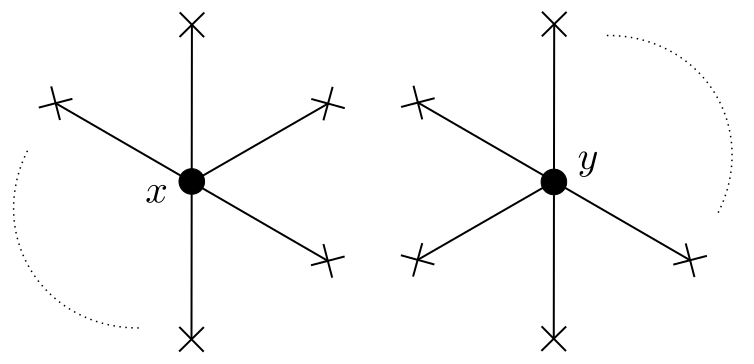
\includegraphics[width=0.65\textwidth]{../pics/tree_level_disconnected_diagram.png}
%
\caption[Disconnected tree-level chiral primary two-point functions]{Disconnected tree-level contribution to the chiral primary two-point functions given in (\ref{the two-point functions}). In the diagram above, the lines with a cross at the end represents insertions of the classical parts, $\mathcal{X}$, $\mathcal{Z}$ and $\bar{\mathcal{Z}}$, of the $\boldsymbol{X}$, $\boldsymbol{Z}$ and $\boldsymbol{\bar{Z}}$ fields respectively.}
%
\label{fig:tree_level_disconnected_diagram}
%
\end{center}
%
\end{figure}
%
%

\subsection{Two-point functions at tree level (\textit{connected})}
At tree level, the two-point functions $\expval{\mathcal{O}_{\boldsymbol{Z}} \, \mathcal{O}_{\boldsymbol{Z}}}$, $\expval{\mathcal{O}_{\boldsymbol{Z}} \, \mathcal{O}_{\boldsymbol{\bar{Z}}}}$ and $\expval{\mathcal{O}_{\boldsymbol{X}} \, \mathcal{O}_{\boldsymbol{Z}}}$ all have only one connected contribution; namely the contribution which arise from Wick-contracting one complex scalar field from the first operator with one complex scalar field from the second.
%
%
\begin{equation}\label{tree-level connected ZZ}
\expval{\tr \boldsymbol{Z}^{L_1} \tr \boldsymbol{Z}^{L_2}}_{\mathrm{tree,c.}}
=
\contraction{L_1 L_2 \tr \big[ \mathcal{Z}^{L_1 - 1} }
{Z}
{ \big] \tr \big[ }
{Z}
L_1 L_2 \tr \big[  \mathcal{Z}^{L_1 - 1} Z \big] 
\tr \big[ Z \mathcal{Z}^{L_2 - 1} \big]
\end{equation}
%
%
\begin{equation}\label{tree-level connected ZbarZ}
\expval{\tr \boldsymbol{Z}^{L_1} \tr \boldsymbol{\bar{Z}}^{L_2}}_{\mathrm{tree,c.}}
=
\contraction{L_1 L_2 \tr \big[ \mathcal{Z}^{L_1 - 1} }
{Z}
{ \big] \tr \big[ }
{\bar{Z}}
L_1 L_2 \tr \big[  \mathcal{Z}^{L_1 - 1} Z \big] 
\tr \big[ \bar{Z} \bar{\mathcal{Z}}^{L_2 - 1} \big]
\end{equation}
%
%
\begin{equation}\label{tree-level connected XZ}
\expval{\tr \boldsymbol{X}^{L_1} \tr \boldsymbol{Z}^{L_2}}_{\mathrm{tree,c.}}
=
\contraction{L_1 L_2 \tr \big[ \mathcal{Z}^{L_1 - 1} }
{X}
{ \big] \tr \big[ }
{Z}
L_1 L_2 \tr \big[  \mathcal{X}^{L_1 - 1} X \big] 
\tr \big[ Z \mathcal{Z}^{L_2 - 1} \big]
\end{equation}
%
%
If any more contractions are made in any way, we obtain loops due to the local nature of the operators. Note that the off-diagonal fields (\textit{w.r.t the decompositions in section} (\ref{diag mass matrix})) do not contribute becuase $\mathcal{Z}$, $\bar{\mathcal{Z}}$ and $\mathcal{X}$ all have no off-diagonal elements. Thus, we only have to consider the upper diagonal parts of $Z$, $\bar{Z}$ and $X$ when doing the contractions.

\subsubsection[$SO(3) \times SO(3)$ symmetric vevs]{$\mathbf{SO(3) \times SO(3)}$ symmetric vevs}
To evaluate the Wick-contractions in the above expressions, we expand the upper diagonal components of $Z$, $\bar{Z}$ and $X$ in a product basis of $\mathfrak{so}(3)$ fussy spherical harmonics, exactly as when we diagonalized the $\mathfrak{so}(3) \times \mathfrak{so}(3)$ symmetric mass matrix back in section \ref{diag mass matrix}.
%
%
\begin{equation}\label{fuzzy harmonic coefficients Z}
Z = Z_{\ell_1,m_1;\ell_2,m_2}
\hat{Y}_{\ell_1}^{m_1} \otimes \hat{Y}_{\ell_2}^{m_2}
\end{equation}
%
%
\begin{equation}\label{fuzzy harmonic coefficients Z bar}
\bar{Z} = Z^\dagger_{\ell_1,m_1;\ell_2,m_2}
(\hat{Y}_{\ell_1}^{m_1})^{\dagger} \otimes (\hat{Y}_{\ell_2}^{m_2})^\dagger
\end{equation}
%
%
\begin{equation}\label{fuzzy harmonic coefficients X}
X = X_{\ell_1,m_1;\ell_2,m_2}
\hat{Y}_{\ell_1}^{m_1} \otimes \hat{Y}_{\ell_2}^{m_2}
\end{equation}
%
%
%\begin{equation}
%Z = Z_{\ell,m;\ell_1, \ell_2}
%\hat{Y}^m_{\ell;\ell_1,\ell_2}
%=
%Z_{\ell,m;\ell_1, \ell_2}
%%\sum_{\ell_1 = 0}^{k_1-1} \sum_{\ell_2 = 0}^{k_2-1}
%\sum_{m_1=-\ell_1}^{\ell_1} \sum_{m_2=-\ell_1}^{\ell_2} \braket{m_1,\ell_1;m_2,\ell_2}{\ell, m; \ell_1, \ell_2} \hat{Y}_{\ell_1}^{m_1} \otimes \hat{Y}_{\ell_2}^{m_2}
%\end{equation}
%%
%%
%\begin{equation}
%Z_{\ell,m;\ell_1, \ell_2} = 
%\sum_{m_1=-\ell_1}^{\ell_1} \sum_{m_2=-\ell_1}^{\ell_2} \braket{m_1,\ell_1;m_2,\ell_2}{\ell, m; \ell_1, \ell_2} Z_{\ell_1,m_1;\ell_2,m_2}
%\end{equation}
%%
%%
The propargators between the coefficient fields above, can now be expressed using the propagators between the scalar coefficient fields $[\phi_i]_{\ell_1,m_1;\ell_2,m_2}$. Since the scalar fields $\phi_i$ are all \textit{complicated}, one must reverse the transformations performed in the process of diagonalizing the complicated mass matrix, in order to obtained these propagators. The details of this reversal can be found in \cite{One-point functions in D3-D7}.\\
Let us now begin to construct the propagators we need to compute the tree-level contribution to the three different two-point functions. Firstly, the relevant $\phi_i$ propagators for computing the contribution (\ref{tree-level connected ZZ}) to $\expval{\mathcal{O}_{Z} \, \mathcal{O}_{Z}}$, are the following ones.
%
%
\begin{equation*}
\expval{
[\phi_3]_{\boldsymbol{\ell}} \,
[\phi_3]_{\boldsymbol{\ell}'}
}
=
(-1)^{m_1' + m_2'} \expval{
[\phi_3]_{\ell_1,m_1;\ell_2,m_2}
[\phi_3]^\dagger_{\ell_1',-m_1';\ell_2',-m_2'}
}
=
(-1)^{m_1' + m_2'}
\end{equation*}
%
%
\begin{equation}\label{phi3-phi3}
\times
\delta_{\ell_1 \ell_1'} \delta_{\ell_2 \ell_2'} \delta_{m_2+m_2',0}
\left[
\delta_{m_1+m_1',0} K^{\phi,(1)}_{\mathrm{sing}}
- [t_3^{(\ell_1)} t_3^{(\ell_1)}]_{m_1, -m_1'} K^{\phi,(1)}_{\mathrm{sym}}
\right]
\end{equation}
%
%

%
%
\begin{equation*}
\expval{
[\phi_6]_{\boldsymbol{\ell}} \,
[\phi_6]_{\boldsymbol{\ell}'}
}
=
(-1)^{m_1' + m_2'} \expval{
[\phi_6]_{\ell_1,m_1;\ell_2,m_2}
[\phi_6]^\dagger_{\ell_1',-m_1';\ell_2',-m_2'}
}
=
(-1)^{m_1' + m_2'}
\end{equation*}
%
%
\begin{equation}\label{phi6-phi6}
\times
\delta_{\ell_1 \ell_1'} \delta_{\ell_2 \ell_2'} \delta_{m_1+m_1',0}
\left[
\delta_{m_2+m_2',0} K^{\phi,(2)}_{\mathrm{sing}}
- [t_3^{(\ell_2)} t_3^{(\ell_2)}]_{m_2, -m_2'} K^{\phi,(2)}_{\mathrm{sym}}
\right]
\end{equation}
%
%

%
%
\begin{equation*}
\expval{
[\phi_3]_{\boldsymbol{\ell}} \,
[\phi_6]_{\boldsymbol{\ell}'}
}
=
(-1)^{m_1' + m_2'} \expval{
[\phi_3]_{\ell_1,m_1;\ell_2,m_2}
[\phi_6]^\dagger_{\ell_1',-m_1';\ell_2',-m_2'}
}
=
(-1)^{m_1' + m_2'}
\end{equation*}
%
%
\begin{equation}\label{phi3-phi6}
\times
\delta_{\ell_1 \ell_1'} \delta_{\ell_2 \ell_2'}
[t_3^{(\ell_1)}]_{m_1, -m_1'} [t_3^{(\ell_2)}]_{m_2, -m_2'} K^{\phi}_{\mathrm{opp}}
\end{equation}
%
%
Where we have introduced the notation $\boldsymbol{\ell} = (\ell_1,m_1;\ell_2,m_2)$, in an attempt to unclutter the notation. Next, the relevant propagators for computing the contribution (\ref{tree-level connected ZbarZ}) to $\expval{\mathcal{O}_{Z} \, \mathcal{O}_{\bar{Z}}}$, are the following.
%
%
\begin{equation}\label{phi3-phibar3}
\expval{
[\phi_3]_{\boldsymbol{\ell}} \,
[\phi_3]^\dagger_{\boldsymbol{\ell}'}
}
=
\delta_{\ell_1 \ell_1'} \delta_{\ell_2 \ell_2'} \delta_{m_2,m_2'}
\left[
\delta_{m_1,m_1'} K^{\phi,(1)}_{\mathrm{sing}}
- [t_3^{(\ell_1)} t_3^{(\ell_1)}]_{m_1, m_1'} K^{\phi,(1)}_{\mathrm{sym}}
\right]
\end{equation}
%
%

%
%
\begin{equation}\label{phi6-phibar6}
\expval{
[\phi_6]_{\boldsymbol{\ell}} \,
[\phi_6]^\dagger_{\boldsymbol{\ell}'}
}
=
\delta_{\ell_1 \ell_1'} \delta_{\ell_2 \ell_2'} \delta_{m_1,m_1'}
\left[
\delta_{m_2,m_2'} K^{\phi,(2)}_{\mathrm{sing}}
- [t_3^{(\ell_2)} t_3^{(\ell_2)}]_{m_2, m_2'} K^{\phi,(2)}_{\mathrm{sym}}
\right]
\end{equation}
%
%

%
%
\begin{equation}\label{phi3-phibar6}
\expval{
[\phi_3]_{\boldsymbol{\ell}} \,
[\phi_6]^\dagger_{\boldsymbol{\ell}'}
}
=
\delta_{\ell_1 \ell_1'} \delta_{\ell_2 \ell_2'}
[t_3^{(\ell_1)}]_{m_1, m_1'} [t_3^{(\ell_2)}]_{m_2, m_2'} K^{\phi}_{\mathrm{opp}}
\end{equation}
%
%
Lastly, the relevant propagators for computing the contribution (\ref{tree-level connected XZ}) to $\expval{\mathcal{O}_{X} \, \mathcal{O}_{Z}}$, are the following.
%
%
\begin{equation*}
\expval{
[\phi_1]_{\boldsymbol{\ell}} \,
[\phi_3]_{\boldsymbol{\ell}'}
}
=
(-1)^{m_1' + m_2'} \expval{
[\phi_1]_{\ell_1,m_1;\ell_2,m_2}
[\phi_3]^\dagger_{\ell_1',-m_1';\ell_2',-m_2'}
}
=
(-1)^{m_1' + m_2'}
\end{equation*}
%
%
\begin{equation}
\times
\delta_{\ell_1 \ell_1'} \delta_{\ell_2 \ell_2'}
\delta_{m_2+m_2',0}
\left[
i \, [t_2^{(\ell_1)}]_{m_1, -m_1'} K^{\phi,(1)}_{\text{anti}}
-
[t_1^{(\ell_1)} t_3^{(\ell_1)}]_{m_1, -m_1'} K^{\phi,(1)}_{\mathrm{sym}}
\right]
\end{equation}
%
%

%
%
\begin{equation*}
\expval{
[\phi_4]_{\boldsymbol{\ell}} \,
[\phi_6]_{\boldsymbol{\ell}'}
}
=
(-1)^{m_1' + m_2'} \expval{
[\phi_4]_{\ell_1,m_1;\ell_2,m_2}
[\phi_6]^\dagger_{\ell_1',-m_1';\ell_2',-m_2'}
}
=
(-1)^{m_1' + m_2'}
\end{equation*}
%
%
\begin{equation}
\times
\delta_{\ell_1 \ell_1'} \delta_{\ell_2 \ell_2'}
\delta_{m_1+m_1',0}
\left[
i \, [t_2^{(\ell_2)}]_{m_2, -m_2'} K^{\phi,(2)}_{\text{anti}}
-
[t_1^{(\ell_2)} t_3^{(\ell_2)}]_{m_2, -m_2'} K^{\phi,(2)}_{\mathrm{sym}}
\right]
\end{equation}
%
%

%
%
\begin{equation*}
\expval{
[\phi_1]_{\boldsymbol{\ell}} \,
[\phi_6]_{\boldsymbol{\ell}'}
}
=
(-1)^{m_1' + m_2'} \expval{
[\phi_1]_{\ell_1,m_1;\ell_2,m_2}
[\phi_6]^\dagger_{\ell_1',-m_1';\ell_2',-m_2'}
}
=
(-1)^{m_1' + m_2'}
\end{equation*}
%
%
\begin{equation}
\times
\delta_{\ell_1 \ell_1'} \delta_{\ell_2 \ell_2'}
[t_1^{(\ell_1)}]_{m_1, -m_1'}
[t_3^{(\ell_2)}]_{m_2, -m_2'}
K^{\phi}_{\text{opp}}
\end{equation}
%
%

%
%
\begin{equation*}
\expval{
[\phi_4]_{\boldsymbol{\ell}} \,
[\phi_3]_{\boldsymbol{\ell}'}
}
=
(-1)^{m_1' + m_2'} \expval{
[\phi_4]_{\ell_1,m_1;\ell_2,m_2}
[\phi_3]^\dagger_{\ell_1',-m_1';\ell_2',-m_2'}
}
=
(-1)^{m_1' + m_2'}
\end{equation*}
%
%
\begin{equation}
\times
\delta_{\ell_1 \ell_1'} \delta_{\ell_2 \ell_2'}
[t_1^{(\ell_2)}]_{m_2, -m_2'}
[t_3^{(\ell_1)}]_{m_1, -m_1'}
K^{\phi}_{\text{opp}}
\end{equation}
%
%
Where in writing down expressions for the above scalar propagators, we have made repeated use of the following property of fuzzy spherical harmonics.
%
%
\begin{equation}
(\hat{Y}^m_\ell)^\dagger
=
(-1)^m \, \hat{Y}^{-m}_\ell
%
\quad \Rightarrow \quad
%
[\phi_i]^\dagger_{\ell_1,m_1;\ell_2,m_2}
=
(-1)^{m_1' + m_2'} \,
[\phi_i]_{\ell_1,-m_1;\ell_2,-m_2}
\end{equation}
%
%
The explicit expressions for the propagators $K^{\phi,(s)}_{\text{sym}}$, $K^{\phi,(s)}_{\text{anti}}$ and $K^{\phi}_{\text{opp}}$ can be found in appendix \ref{app:complex propagators}, and the matrix elements of the $\mathfrak{su}(2)$ generators $[t^{(\ell)}_i]_{m,m'} \equiv \bra{\ell, m} t^{(\ell)}_i \ket{\ell, m'}$, are given by the following standard expressions.

\newpage
%
%
\begin{equation}\label{so(3) generators 1}
[t^{(\ell)}_1]_{m,m'}
=
\frac{1}{2} \left(
C^\ell_{m,m'} \delta_{m',m-1}
+ 
C^\ell_{m',m} \delta_{m',m+1}
\right)
\end{equation}
%
%
\begin{equation}\label{so(3) generators 2}
[t^{(\ell)}_2]_{m,m'}
=
\frac{1}{2 i} \left(
C^\ell_{m,m'} \delta_{m',m-1}
- 
C^\ell_{m',m} \delta_{m',m+1}
\right)
\end{equation}
%
%
\begin{equation}\label{so(3) generators 3}
[t^{(\ell)}_3]_{m,m'}
=
m \, \delta_{m',m}
%
\quad , \quad
%
C^\ell_{m,m'} = \sqrt{(\ell+m)(\ell-m')}
\end{equation}
%
%
Using all the scalar propagators written above, we can easily find the propergators: $\langle Z_{\boldsymbol{\ell}} \, Z_{\boldsymbol{\ell}'} \rangle$, $\langle Z_{\boldsymbol{\ell}} \, Z^\dagger_{\boldsymbol{\ell}'} \rangle$ and $\langle X_{\boldsymbol{\ell}} \, Z_{\boldsymbol{\ell}'} \rangle$, by simply using definition (\ref{chiral_primaries}) and expanding the products appearing in the propagators. The results are given below.
%
%
\begin{equation}
\langle
Z_{\boldsymbol{\ell}} \, Z_{\boldsymbol{\ell}'}
\rangle
=
\expval{
[\phi_3]_{\boldsymbol{\ell}} \,
[\phi_3]_{\boldsymbol{\ell}'}
}
- \expval{
[\phi_6]_{\boldsymbol{\ell}} \,
[\phi_6]_{\boldsymbol{\ell}'}
}
+ i \left(
\expval{
[\phi_3]_{\boldsymbol{\ell}} \,
[\phi_6]_{\boldsymbol{\ell}'}
}
+
\expval{
[\phi_6]_{\boldsymbol{\ell}} \,
[\phi_3]_{\boldsymbol{\ell}'}
}
\right)
\end{equation}
%
%
\begin{equation}
\langle
Z_{\boldsymbol{\ell}} \, Z^\dagger_{\boldsymbol{\ell}'}
\rangle
=
\expval{
[\phi_3]_{\boldsymbol{\ell}} \,
[\phi_3]^\dagger_{\boldsymbol{\ell}'}
}
+
\expval{
[\phi_6]_{\boldsymbol{\ell}} \,
[\phi_6]^\dagger_{\boldsymbol{\ell}'}
}
+ i \left(
\expval{
[\phi_6]_{\boldsymbol{\ell}} \,
[\phi_3]^\dagger_{\boldsymbol{\ell}'}
}
-
\expval{
[\phi_3]_{\boldsymbol{\ell}}
[\phi_6]^\dagger_{\boldsymbol{\ell}'}
}
\right)
\end{equation}
%
%
\begin{equation}
\langle
X_{\boldsymbol{\ell}} \, Z_{\boldsymbol{\ell}'}
\rangle
=
\expval{
[\phi_1]_{\boldsymbol{\ell}} \,
[\phi_3]_{\boldsymbol{\ell}'}
}
-
\expval{
[\phi_4]_{\boldsymbol{\ell}} \,
[\phi_6]_{\boldsymbol{\ell}'}
}
+ i \left(
\expval{
[\phi_4]_{\boldsymbol{\ell}} \,
[\phi_3]_{\boldsymbol{\ell}'}
}
+
\expval{
[\phi_1]_{\boldsymbol{\ell}} \,
[\phi_6]_{\boldsymbol{\ell}'}
}
\right)
\end{equation}
%
%
If we now insert the explicit forms of the $\phi_i$ field propagators into the above expressions and make use of (\ref{so(3) generators 1}), (\ref{so(3) generators 2}) and (\ref{so(3) generators 3}), we find that the complex scalar propagators simplify quite a lot. For $\langle
Z_{\boldsymbol{\ell}} \, Z_{\boldsymbol{\ell}'}
\rangle$, we find that.
\begin{equation*}
\langle
Z_{\boldsymbol{\ell}} \, Z_{\boldsymbol{\ell}'}
\rangle
=
(-1)^{m_1' + m_2'} \,
\delta_{\ell_1 \ell_1'} \delta_{\ell_2 \ell_2'}
\delta_{m_1+m_1',0} \delta_{m_2 + m_2',0}
\end{equation*}
%
%
\begin{equation}\label{ZZ propagotor}
\times
\left.
\left[
K^{\phi,(1)}_{\mathrm{sing}} - K^{\phi,(2)}_{\mathrm{sing}}
- m_1^2 K^{\phi,(1)}_{\mathrm{sym}}
+ m_2^2 K^{\phi,(2)}_{\mathrm{sym}}
+ 2i m_1 m_2 K^{\phi}_{\mathrm{opp}}
\right]
\right\rbrace { \scriptstyle K^{ZZ} }
\end{equation}
%
%
For $\langle Z_{\boldsymbol{\ell}} \, Z^\dagger_{\boldsymbol{\ell}'} \rangle$, we find that.
%
%
\begin{equation*}
\langle
Z_{\boldsymbol{\ell}} \, Z^\dagger_{\boldsymbol{\ell}'}
\rangle
=
\delta_{\ell_1 \ell_1'} \delta_{\ell_2 \ell_2'}
\delta_{m_1 m_1'} \delta_{m_2 m_2'}
\end{equation*}
%
%
\begin{equation}\label{ZbarZ propagotor}
\times
\left.
\left[
K^{\phi,(1)}_{\mathrm{sing}} + K^{\phi,(2)}_{\mathrm{sing}}
- m_1^2 K^{\phi,(1)}_{\mathrm{sym}}
- m_2^2 K^{\phi,(2)}_{\mathrm{sym}}
\right]
\right\rbrace { \scriptstyle K^{Z\bar{Z}} }
\end{equation}
%
%
For $\langle X_{\boldsymbol{\ell}} \, Z_{\boldsymbol{\ell}'} \rangle$, we find that.
%
%
\begin{equation*}
\langle
X_{\boldsymbol{\ell}} \, Z_{\boldsymbol{\ell}'}
\rangle
=
\frac{1}{2} (-1)^{m_1' + m_2'} \,
\delta_{\ell_1 \ell_1'} \delta_{\ell_2 \ell_2'}
\end{equation*}
%
%
\begin{equation*}
\times
\delta_{m_2 + m_2',0} \delta_{m_1 + m_1',1} C^{\ell_1}_{m_1,-m_1'}
\left.
\left[
K^{\phi,(1)}_{\text{anti}}
+
m_1' K^{\phi,(1)}_{\text{sym}}
-
i \, m_2' K^{\phi}_{\text{opp}}
\right]
\right\rbrace { \scriptstyle K^{XZ}_{(1),+} }
\end{equation*}
%
%
\begin{equation*}
\times
\delta_{m_2 + m_2',0} \delta_{m_1 + m_1',-1} C^{\ell_1}_{-m_1',m_1}
\left.
\left[
-
K^{\phi,(1)}_{\text{anti}}
+
m_1' K^{\phi,(1)}_{\text{sym}}
-
i \, m_2' K^{\phi}_{\text{opp}}
\right]
\right\rbrace { \scriptstyle K^{XZ}_{(1),-} }
\end{equation*}
%
%
\begin{equation*}
\times
\delta_{m_1 + m_1',0} \delta_{m_2 + m_2',1} C^{\ell_2}_{m_2,-m_2'}
\left.
\left[
-
K^{\phi,(2)}_{\text{anti}}
-
m_2' K^{\phi,(2)}_{\text{sym}}
-
i \, m_1' K^{\phi}_{\text{opp}}
\right]
\right\rbrace { \scriptstyle K^{XZ}_{(2),+} }
\end{equation*}
%
%
\begin{equation}\label{XZ propagotor}
\times
\delta_{m_1 + m_1',0} \delta_{m_2 + m_2',-1} C^{\ell_2}_{-m_2',m_2}
\left.
\left[
K^{\phi,(2)}_{\text{anti}}
-
m_2' K^{\phi,(2)}_{\text{sym}}
-
i \, m_1' K^{\phi}_{\text{opp}}
\right]
\right\rbrace { \scriptstyle K^{XZ}_{(2),-} }
\end{equation}
%
%

\newpage
Now that we have expressions for all the relevant propagators between the complex scalar coefficient fields, we can attempt to compute the leading order connected contribution to the two-point functions $\expval{\mathcal{O}_{\boldsymbol{Z}} \, \mathcal{O}_{\boldsymbol{Z}}}$, $\expval{\mathcal{O}_{\boldsymbol{Z}} \, \mathcal{O}_{\boldsymbol{\bar{Z}}}}$ and $\expval{\mathcal{O}_{\boldsymbol{X}} \, \mathcal{O}_{\boldsymbol{Z}}}$. We start out by considering the constribution (\ref{tree-level connected ZZ}) to $\expval{\mathcal{O}_{\boldsymbol{Z}} \, \mathcal{O}_{\boldsymbol{Z}}}$.
%
%
\begin{equation*}
\expval{\tr \boldsymbol{Z}^{L_1+1} \tr \boldsymbol{Z}^{L_2+1}}_{\mathrm{tree,c.}}
=
\frac{(-1)^{L_1 + L_2} (L_1+1) (L_2+1)}{x_3^{L_1} y_3^{L_2}}
\langle
Z_{\boldsymbol{\ell}} \, Z_{\boldsymbol{\ell}'}
\rangle
\end{equation*}
%
%
\begin{equation}\label{ZZ c. two-point}
\tr[(t^{(1)}_3 + i \, t^{(2)}_3)^{L_1} \, \hat{Y}_{\ell_1}^{m_1} \otimes \hat{Y}_{\ell_2}^{m_2}]
\tr[(t^{(1)}_3 + i \, t^{(2)}_3)^{L_2} \, \hat{Y}_{\ell_1'}^{m_1'} \otimes \hat{Y}_{\ell_2'}^{m_2'}]
\end{equation}
%
%
Where we have used the notation of section \ref{sec:dCFT}; $t^{(1)}_i \equiv t^{k_1}_i \otimes \mathbb{1}_{k_2}$ and $t^{(2)}_i \equiv \mathbb{1}_{k_1} \otimes t^{k_2}_i$. To proceed further, we now rewrite the products appearing in the traces above as binomial expansions.
%
%
\begin{equation}\label{binomial sum}
\tr[(t^{(1)}_3 + i \, t^{(2)}_3)^{L} \, \hat{Y}_{\ell_1}^{m_1} \otimes \hat{Y}_{\ell_2}^{m_2}]
=
\sum_{p=0}^{L}
\binom{L}{p} i^{p}
\tr \big[ (t_3^{k_1})^{L - p} \, \hat{Y}_{\ell_1}^{m_1} \otimes (t_3^{k_2})^{p} \, \hat{Y}_{\ell_2}^{m_2} \big]
\end{equation}
%
%
The traces of the $\mathfrak{so}(3)$ generators $t_3^{k_s}$ with the fuzzy spherical harmonics $\hat{Y}_{\ell}^{m}$ now have to be evaluated somehow. This was first done in \cite{Two-point functions in D5-D3}, by taking advantage of certain properties of the fuzzy spherical harmonics. The result of the whole procedure is the following.
%
%
\begin{equation*}
\tr \big[ (t_3^{k_1})^{p_1} \, \hat{Y}_{\ell_1}^{m_1} \otimes (t_3^{k_2})^{p_2} \, \hat{Y}_{\ell_2}^{m_2} \big]
=
\tr \big[ (t_3^{k_1})^{p_1} \, \hat{Y}_{\ell_1}^{m_1} \big]
\tr \big[ (t_3^{k_2})^{p_2} \, \hat{Y}_{\ell_2}^{m_2} \big]
\end{equation*}
%
%
\begin{equation}\label{alpha trace}
=
\alpha_{\ell_1;k_1}^{p_1} \alpha_{\ell_2;k_2}^{p_2}
\delta^{m_1,0} \delta^{m_2,0}
\end{equation}
%
%

%
%
\begin{equation}\label{alpha not reduced}
\alpha_{m;k}^L
\simeq
(-1)^k \, 
\left( \frac{k}{2} \right)^{L + \frac{1}{2}} \, 
i^m \, \sqrt{m + \frac{1}{2}} \,
\begin{cases}
		\frac{1}{L+1}
		\frac{\left( \frac{2-L}{2} \right)_{\frac{m-2}{2}}}
		{\left( \frac{L+3}{2} \right)_{\frac{m}{2}}}
		& \quad \text{for } L,m \text{ even} \\
		
    	i
		\frac{\left( \frac{1-L}{2} \right)_{\frac{m-1}{2}}}
		{\left( \frac{L+2}{2} \right)_{\frac{m+1}{2}}}
    	& \quad \text{for } L,m \text{ odd}
  \end{cases}
\end{equation}
%
%
Where in this context, $\simeq$ means equal to highest order in $k$, Furthermore, $\alpha_{m;k}^L$ will evaluate to zero if certain conditions are not met. These conditions can be found below.
%
%
\begin{enumerate}
%
\item Both $L$ and $m$ was to be either even or odd.
%
\item The inequality $L \geq m$ has to be satisfied.
%
\end{enumerate}
%
%
It turns out that it is possible to bring (\ref{alpha not reduced}) to a form which is much more symmetric between the $L$, $m$ even and $L$, $m$ odd cases. This more symmetric form looks as follow.
%
%
\begin{equation*}
\alpha_{m;k}^L
\simeq
(-1)^{k + m} \, 
\left( \frac{k}{2} \right)^{L + \frac{1}{2}} \,
\frac{\sqrt{\pi \left( m + \frac{1}{2} \right)}}{2^L}
\end{equation*}
%
%
\begin{equation}
\times
\frac{\Gamma(L+1)}
{
\Gamma \left( \frac{L+m+3}{2} \right) \,
\Gamma \left( \frac{L-m+2}{2} \right)
}
\begin{cases}
		-1
		& \quad \text{for } L,m \text{ even} \\
		
    	1
    	& \quad \text{for } L,m \text{ odd}
  \end{cases}
\end{equation}
%
%
%
%
%%
%%
%\begin{equation}
%\log
%\left[
%\frac
%{
%\Gamma(L + 1)
%}
%{
%\Gamma \left( \frac{L-p+\ell_1+3}{2} \right)
%\Gamma \left( \frac{L-p-\ell_1+2}{2} \right)
%\Gamma \left( \frac{p+\ell_2+3}{2} \right)
%\Gamma \left( \frac{p-\ell_2+2}{2} \right)
%}
%\right]
%\end{equation}
%%
%%
%\begin{equation}
%=
%\log
%\left[
%\frac
%{
%2^{q_{1,+} + q_{2,+}} \, L!
%}
%{
%\pi \,
%q_{1,-}! \, q_{2,-}! \,
%(2 q_{1,+} + 1)!! \, (2 q_{2,+} + 1)!!
%}
%\right]
%\end{equation}
%%
%%
%\begin{equation}
%=
%(q_{1,+} + q_{2,+}) \log[2]
%+
%\log[L!]
%-
%\log[\pi]
%\end{equation}
%%
%%
%\begin{equation}
%-
%\log
%\left[
%q_{1,-}!
%\right]
%-
%\log
%\left[
%q_{2,-}!
%\right]
%-
%\log
%\left[
%(2 q_{1,+} + 1)!!
%\right]
%-
%\log
%\left[
%(2 q_{2,+} + 1)!!
%\right]
%\end{equation}
%%
%%
%\begin{equation}
%q_{1,\pm} \equiv \frac{L - p \pm \ell_1}{2} \in \mathbb{N}_0
%%
%\quad , \quad
%%
%q_{2,\pm} \equiv \frac{p \pm \ell_2}{2} \in \mathbb{N}_0
%\end{equation}
%%
%%
We now need to evaluate the sum (\ref{binomial sum}). For given $L$, $\ell_1$ and $\ell_2$, this would be a straightforward computation. For example, in the case of $L=2$, $\ell_1 = 0$ and $\ell_2 = 0$ the sum (\ref{binomial sum}) evaluates to following simple expression. 
%
%
\begin{equation}
\sum_{p=0}^{2}
i^p
\binom{L}{p}
\alpha_{\ell_1=0;k_1}^{2-p} \alpha_{\ell_2=0;k_2}^{p}
=
\frac{(-1)^{k_1 + k_2 + 1}}{12} \, \left[
k_1^{1/2} k_2^{5/2}
-
k_2^{5/2} k_2^{1/2}
\right]
\end{equation}
%
%
Where we have omitted the factor of $\delta^{m_1,0} \delta^{m_2,0}$. For general $L$, $\ell_1$ and $\ell_2$, we were not able to find an explicit expression for the sum (\ref{binomial sum}), due to the fact that we can not know which terms in the sum are non-zero apriori. This is because of the conditions $L-p \geq \ell_1$ and $p \geq \ell_2$. From the exact same conditions (\textit{together with the parity conditions}), we can however obtain some general conditions on the sum (\ref{binomial sum}).
%
%
\begin{align}\label{binomial sum conditions}
\sum_{p=0}^{L}
i^p
\binom{L}{p}
\alpha_{\ell_1;k_1}^{L-p} \alpha_{\ell_2;k_2}^{p}
=
0
%
\quad \text{unless} \quad
%
L + \ell_1 + \ell_2
\text{ even, and }
L \geq \ell_1 + \ell_2
\end{align}
%
%
Now that we have a better understanding of the traces which appear in (\ref{ZZ c. two-point}), we can continue the evaluation of this connected contribution to $\expval{\mathcal{O}_{\boldsymbol{Z}} \, \mathcal{O}_{\boldsymbol{Z}}}$. By inserting (\ref{ZZ propagotor}), (\ref{binomial sum}) and (\ref{alpha trace}) into (\ref{ZZ c. two-point}), we find the following expression for the connected tree-level contribution to $\expval{\mathcal{O}_{\boldsymbol{Z}} \, \mathcal{O}_{\boldsymbol{Z}}}$.
%
%
\begin{equation*}
\expval{\tr \boldsymbol{Z}^{L_1+1} \tr \boldsymbol{Z}^{L_2+1}}_{\mathrm{tree,c.}}
\simeq
\frac{(L_1+1) (L_2+1)}{x_3^{L_1} y_3^{L_2}}
\end{equation*}
%
%
\begin{equation}\label{evil sum}
\times
\sum_{\ell_1=0}^{k_1-1}
\sum_{\ell_2=0}^{k_2-1}
\left[
K^{\phi,(1)}_{\mathrm{sing}}
- K^{\phi,(2)}_{\mathrm{sing}}
\right]
\sum_{p_1=0}^{L_1} i^{p_1}
\binom{L_1}{p_1}
\alpha_{\ell_1;k_1}^{L_1-p_1} \alpha_{\ell_2;k_2}^{p_1}
\sum_{p_2=0}^{L_2} i^{p_2}
\binom{L_2}{p_2}
\alpha_{\ell_1;k_1}^{L_2-p_2} \alpha_{\ell_2;k_2}^{p_2}
\end{equation}
%
%
Note that the factor of $(-1)^{L_1 + L_2}$ present in (\ref{ZZ c. two-point}) drops out due to the properties of $\alpha_{m;k}^L$. Since we do not know general expressions for the (\ref{binomial sum conditions}) type sums, we do not at the moment of writing this know how to evaluate the above expression for arbitrary $L_1$, $L_2$ and $k_2$, $k_1$. The sums can however be evaluated numerically for any values of the parameters $L_1$, $L_2$ and $k_2$, $k_1$. See for example table \ref{tab:ZZ_two_point_functions_so(3)}. The sums can also be evaluated analytically for some particularly simple values of the parameters, which we will explore further shortly. Before we do so however, let us write down reduced expressions for the connected contributions to $\expval{\mathcal{O}_{\boldsymbol{Z}} \, \mathcal{O}_{\boldsymbol{\bar{Z}}}}$ and $\expval{\mathcal{O}_{\boldsymbol{X}} \, \mathcal{O}_{\boldsymbol{Z}}}$. For $\expval{\mathcal{O}_{\boldsymbol{Z}} \, \mathcal{O}_{\boldsymbol{\bar{Z}}}}$, we find something very similar to (\ref{evil sum}).
%
%
\begin{equation*}
\expval{\tr \boldsymbol{Z}^{L_1+1} \tr \boldsymbol{\bar{Z}}^{L_2+1}}_{\mathrm{tree,c.}}
\simeq
\frac{(L_1 + 1) (L_2 + 1)}{x_3^{L_1} y_3^{L_2}}
\end{equation*}
%
%
\begin{equation}
\times
\sum_{\ell_1=0}^{k_1-1}
\sum_{\ell_2=0}^{k_2-1}
\left[
K^{\phi,(1)}_{\mathrm{sing}}
+ K^{\phi,(2)}_{\mathrm{sing}}
\right]
\sum_{p_1=0}^{L_1} i^{p_1}
\binom{L_1}{p_1}
\alpha_{\ell_1;k_1}^{L_1-p_1} \alpha_{\ell_2;k_2}^{p_1}
\sum_{p_2=0}^{L_2} (-i)^{p_2}
\binom{L_2}{p_2}
\alpha_{\ell_1;k_1}^{L_2-p_2} \alpha_{\ell_2;k_2}^{p_2}
\end{equation}
%
%
Similarly to the $\expval{\mathcal{O}_{\boldsymbol{Z}} \, \mathcal{O}_{\boldsymbol{Z}}}$ case, we were not able to obtain a closed expression for general parameter values, but numerical results can easily be obtained. See for example table \ref{tab:ZbarZ_two_point_functions_so(3)}. Lastly, we write down the reduced expressions for the connected contributions to $\expval{\mathcal{O}_{\boldsymbol{X}} \, \mathcal{O}_{\boldsymbol{Z}}}$. To do this, we will need following relation between the traces $\tr[(t_1^k)^p \, \hat{Y}^m_\ell]$ and $\tr[(t_3^k)^p \, \hat{Y}^0_\ell]$, which was worked out in \cite{Two-point functions in D5-D3}.
%
%
\begin{equation}\label{t1 with fuzzy harmonic trace}
\tr[(t_1^k)^p \, \hat{Y}^m_\ell]
=
\frac{i^{\ell+m}}{2^\ell}
\sqrt{\frac{\Gamma(\ell + m + 1)}{\Gamma(\ell-m+1)}}
\frac{\Gamma(\ell-m+1)}
{
\Gamma \left( \frac{\ell-m+2}{2} \right)
\Gamma \left( \frac{\ell+m+2}{2} \right)
}
\tr[(t_3^k)^p \, \hat{Y}^0_\ell]
\end{equation}
%
%
The relation above is valid for $L,\ell,m$ all even, or $L,\ell,m$ all odd, otherwise the RHS should be set to zero. Because of the structure of $\expval{X_{\boldsymbol{\ell}} \, Z_{\boldsymbol{\ell}'}}$, the cases of $m=\pm 1$ are of particuar interest, and we write these explicitly below.
%
%
\begin{equation}
\tr[(t_1^k)^p \, \hat{Y}^{\pm 1}_\ell]
=
\frac{i^{\ell \pm 1}}{2^\ell}
\sqrt{\frac{\ell + 1}{\ell}}
\binom{\ell}{\frac{\ell-1}{2}}
\tr[(t_3^k)^p \, \hat{Y}^0_\ell]
\end{equation}
%
%
We can now use the above trace relations together with (\ref{XZ propagotor}) and (\ref{alpha trace}), to write down the tree-level connected contribution to the two-point function $\expval{\mathcal{O}_{\boldsymbol{Z}} \, \mathcal{O}_{\boldsymbol{\bar{Z}}}}$. When doing this, we notice the following simplifying observation about the traces.
%
%
\begin{equation*}
C^\ell_{0,-1} \tr[(t_1^k)^p \, \hat{Y}^{+1}_\ell]
=
-C^\ell_{1,0} \tr[(t_1^k)^p \, \hat{Y}^{-1}_\ell]
\end{equation*}
%
%
\begin{equation}
=
\frac{i^{\ell + 1}}{2^\ell}
(\ell + 1)
\binom{\ell}{\frac{\ell-1}{2}}
\tr[(t_3^k)^p \, \hat{Y}^0_\ell]
\end{equation}
%
%
Using the above, we find the following expression for the connected tree-level contribution to $\expval{\mathcal{O}_{\boldsymbol{X}} \, \mathcal{O}_{\boldsymbol{Z}}}$.
%
%
\begin{equation*}
\expval{\tr \boldsymbol{X}^{L_1+1} \tr \boldsymbol{Z}^{L_2+1}}_{\mathrm{tree,c.}}
\simeq
-\frac{(L_1 + 1) (L_2 + 1)}{x_3^{L_1} y_3^{L_2}}
\sum_{\ell_1=1}^{k_1-1}
\sum_{\ell_2=1}^{k_2-1}
\left[
\frac{i^{\ell_1+1}
(\ell_1 + 1)!}
{2^{\ell_1}
\left( \frac{\ell_1 - 1}{2} \right)!
\left( \frac{\ell_1 + 1}{2} \right)!}
K^{\phi,(1)}_{\mathrm{anti}}
\right.
\end{equation*}
%
%
\begin{equation}
\left.
-
\frac{i^{\ell_2+1}
(\ell_2 + 1)!}
{2^{\ell_2}
\left( \frac{\ell_2 - 1}{2} \right)!
\left( \frac{\ell_2 + 1}{2} \right)!}
K^{\phi,(2)}_{\mathrm{anti}}
\right]
\sum_{p_1=0}^{L_1} i^{p_1}
\binom{L_1}{p_1}
\alpha_{\ell_1}^{L_1-p_1} \alpha_{\ell_2}^{p_1}
\sum_{p_2=0}^{L_2} i^{p_2}
\binom{L_2}{p_2}
\alpha_{\ell_1}^{L_2-p_2} \alpha_{\ell_2}^{p_2}
\end{equation}
%
%
For examples of numerical evaluations of $\expval{\mathcal{O}_{\boldsymbol{X}} \, \mathcal{O}_{\boldsymbol{Z}}}$ for some particular $L_1$, $L_2$ and $k_1$, $k_2$, see tab. \ref{tab:XZ_two_point_functions_so(3)}.\\
As was also the case for the other tree-level connected contributions, we do not know whether or not it is possible to explicitly evaluate the sums over $p_1$, $p_2$ and $\ell_1$, $\ell_2$, appearing in the above expression. We suspect that at least part of the difficulty lies with the fact that the masses of the fields are complicated. More specifically, we find that for general $\ell_1$ and $\ell_2$.
%
%
\begin{equation}
\nu = \sqrt{m^2 + \frac{1}{4}} \notin \mathbb{N}_0
\end{equation}
%
%
Where $m^2$ refers to the masses in table \ref{tab:boson_masses_complicated}. That $\nu$ is typically not an integer means that we have square roots appearing in the sums over $\ell_1$ and $\ell_2$, which complicates the evaluation. This hindrance, together with that of the complicated binomial sums, makes it seem unlikely that more explicit expressions for the connected tree-level contributions can be obtained (\textit{at least using the approach of this thesis}).\\
\\
%%
%%
%\begin{equation*}
%K^{\phi,(1)}_{\mathrm{sing}} = \frac{\ell_1 + 1}{2 \ell_1 + 1} K^{m^2_{(1),+}}
%+ \frac{\ell_1}{2 \ell_1 + 1} K^{m^2_{(1),-}}
%\end{equation*}
%%
%%
%\begin{equation*}
%=
%\frac{g^2}{16 \pi^2 x_3 y_3} \left[
%\frac{\ell_1 + 1}{2 \ell_1 + 1} \binom{2 \nu_{(1),+} + 1}{\nu_{(1),+} + \frac{1}{2}}^{-1}
%\frac{{}_2F_1 \left(
%\nu_{(1),+} - \frac{1}{2}, \nu_{(1),+} + \frac{1}{2}; 2 \nu_{(1),+} + 1; -\xi^{-1}
%\right) }
%{(1 + \xi) \xi^{\nu_{(1),+} + \frac{1}{2}} }
%\right.
%\end{equation*}
%%
%%
%\begin{equation}
%\left.
%\frac{\ell_1}{2 \ell_1 + 1} \binom{2 \nu_{(1),-} + 1}{\nu_{(1),-} + \frac{1}{2}}^{-1}
%\frac{{}_2F_1 \left(
%\nu_{(1),-} - \frac{1}{2}, \nu_{(1),-} + \frac{1}{2}; 2 \nu_{(1),-} + 1; -\xi^{-1}
%\right) }
%{(1 + \xi) \xi^{\nu_{(1),-} + \frac{1}{2}} }
%\right]
%\end{equation}
%%
%%
%In principle there would be 1-loop corrections from the 1-loop renormalization of $\tr[Z^J]$ and from the 2-loop wavefunction $\mathcal{O}^{i_1 i_2 \dots i_J}$, but since $\tr[Z^J]$ is a chiral primary, these contributions vanish.
%%
%%
%\begin{equation}
%\expval{
%\tr[Z^{J_1}] \tr[Z^{J_2}]
%}_{\mathrm{lolipop}}
%=
%J_1 \expval{
%\tr[(\phi_3 + i \phi_6) (\mathcal{Z})^{J_1-1}] 
%}
%\tr[(\mathcal{Z})^{J_2}]
%\end{equation}
%%
%%
%\begin{equation}
%+ J_2 \tr[(\mathcal{Z})^{J_1}]
%\expval{
%\tr[(\phi_3 + i \phi_6) (\mathcal{Z})^{J_2-1}]
%}
%\end{equation}
%%
%%
%
%%
%%
%\begin{equation}
%\expval{
%\tr[Z^{J_1}] \tr[Z^{J_2}]
%}_{\mathrm{tadpole}}
%=
%J_1 J_2 \expval{
%\tr[(\phi_3 + i \phi_6) (\mathcal{Z})^{J_1-1}]
%\tr[(\phi_3 + i \phi_6) (\mathcal{Z})^{J_2-1}] 
%}
%\end{equation}
%%
%%
%\begin{equation}
%+ J_1 \sum_{m=0}^{J_1-2}
%\expval{
%\tr[(\phi_3 + i \phi_6)
%(\mathcal{Z})^{m}
%(\phi_3 + i \phi_6)
%(\mathcal{Z})^{J_1-2-m}]
%}
%\tr[(\mathcal{Z})^{J_2}]
%\end{equation}
%%
%%
%\begin{equation}
%+ J_2 \tr[(\mathcal{Z})^{J_1}]
%\sum_{m=0}^{J_2-2}
%\expval{
%\tr[(\phi_3 + i \phi_6)
%(\mathcal{Z})^{m}
%(\phi_3 + i \phi_6)
%(\mathcal{Z})^{J_2-2-m}]
%}
%\end{equation}
%%
%%
%\subsubsection{The case of $\mathbf{J_1 = 1}$ and $\mathbf{J_2 = 1}$}
%
%%
%%
%\begin{equation*}
%\expval{\tr Z(x) \tr \bar{Z}(y)}_{\mathrm{tree,c.}}
%=
%\expval{
%Z_{\ell_1,m_1;\ell_2,m_2}(x)
%\bar{Z}_{\ell_1',m_1';\ell_2',m_2'}(y)
%}
%\end{equation*}
%%
%%
%\begin{equation}
%\times
%\tr \big[ \hat{Y}_{\ell_1}^{m_1} \otimes \hat{Y}_{\ell_2}^{m_2} \big] 
%\tr \big[ \hat{Y}_{\ell_1'}^{m_1'} \otimes \hat{Y}_{\ell_2'}^{m_2'} \big]
%\end{equation}
%%
%%
%
%%
%%
%\begin{equation}
%\tr[\hat{Y}_\ell^m]
%=
%(-1)^{k+1} \sqrt{k} \delta_{m,0} \delta_{\ell,0}
%\end{equation}
%%
%%
%
%%
%%
%\begin{equation*}
%\expval{\tr Z(x) \tr \bar{Z}(y)}_{\mathrm{tree,c.}}
%=
%\frac{g^2}{x_3 y_3} k^2 K^{m^2 = 0}
%=
%\frac{g^2}{x_3 y_3} k^2 K^{\nu = 1/2}
%\sim
%\xi^{-1} - 1 + \xi - \xi^2 + \dots
%\end{equation*}
%%
%%

%%
%%
%\begin{equation*}
%\expval{\tr Z^{J_1}(x) \tr Z^{J_2}(y)}_{\mathrm{tree,c.}}
%=
%\frac{(-1)^{J_1 + J_2} J_1 J_2}{x_3^{J_1-1} y_3^{J_2-1}}
%\expval{
%Z_{\ell,m;\ell_1,\ell_2}(x)
%Z_{\ell',m';\ell_1',\ell_2'}(y)
%}
%\end{equation*}
%%
%%
%\begin{equation}
%\times
%\tr[t_3^{J_1-1} \hat{Y}^m_{\ell; \ell_1,\ell_2}]
%\tr[t_3^{J_2-1} \hat{Y}^{m'}_{\ell'; \ell_1',\ell_2'}]
%\end{equation}
%%
%%
%%
%%
%\begin{figure}
%    \centering
%    \begin{subfigure}[b]{0.49\textwidth}
%        \includegraphics[width=\textwidth]{../pics/beta_L=100.png}
%        \caption{Graph of $\beta(L=100,p,\ell_1=0,\ell_2=0)$.}
%        \label{fig:beta_L=100}
%    \end{subfigure}
%    ~ %add desired spacing between images, e. g. ~, \quad, \qquad, \hfill etc. 
%      %(or a blank line to force the subfigure onto a new line)
%    \begin{subfigure}[b]{0.49\textwidth}
%        \includegraphics[width=\textwidth]{../pics/beta_L=500.png}
%        \caption{Graph of $\beta(L=500,p,\ell_1=0,\ell_2=0)$.}
%        \label{fig:beta_L=500}
%    \end{subfigure}
%    \caption{Graph of $\beta(L,p,\ell_1=0,\ell_2=0)$ for $L = 100,500$. The numerical evidence seem to suggest that $\beta(L,p,\ell_1=0,\ell_2=0)$ peaks at the value $p=L/2$, and that the peak width decreases proportionally as $L$ increases.}\label{fig:beta}
%\end{figure}
%%
%%
%
%
\begin{figure}
%
\begin{center}
%
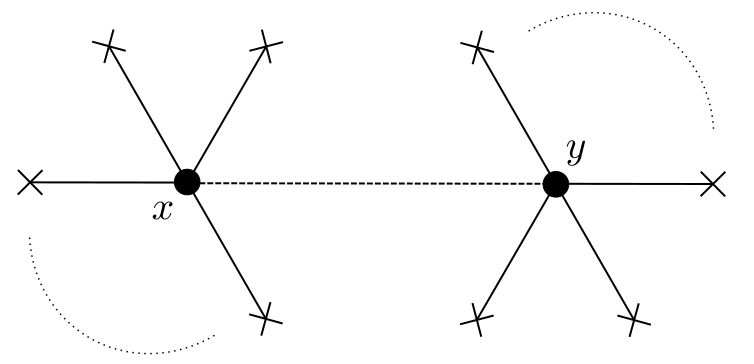
\includegraphics[width=0.65\textwidth]{../pics/tree_level_connected_diagram.png}
%
\caption[Connected tree-level chiral primary two-point functions]{Connected tree-level contribution to the chiral primary two-point functions given in (\ref{the two-point functions}). In the diargram above, the lines with a cross at the end represents insertions of the classical parts, $\mathcal{X}$, $\mathcal{Z}$ and $\bar{\mathcal{Z}}$, of the $\boldsymbol{X}$, $\boldsymbol{Z}$ and $\boldsymbol{\bar{Z}}$ fields respectively. The doted line represents either a $\expval{X_{\boldsymbol{\ell}} \, Z_{\boldsymbol{\ell}'}}$, $\expval{Z_{\boldsymbol{\ell}} \, Z_{\boldsymbol{\ell}'}}$ or $\langle Z_{\boldsymbol{\ell}} \, Z^\dagger_{\boldsymbol{\ell}'} \rangle$ propagator.}
%
\label{fig:tree_level_connected_diagram}
%
\end{center}
%
\end{figure}
%
%

\paragraph[The case of $L_1 = 2$ and $L_2 = 2$]{The case of $\mathbf{L_1 = 2}$ and $\mathbf{L_2 = 2}$:}
One of the special cases in which the connected tree-level contributions to the two-point functions (\ref{the two-point functions}) can be evaluated explicitly, is whenever we have $L_1 = L_2 = 2$ and $k_1$, $k_2$ arbitrary. In this case, the expression (\ref{evil sum}) for the connected contribution to $\expval{\mathcal{O}_{\boldsymbol{Z}} \mathcal{O}_{\boldsymbol{Z}}}$ reduces to the following.
%
%
\begin{equation*}\label{connected contribution ZZ L1=L2=1}
\expval{\tr \boldsymbol{Z}^2 \tr \boldsymbol{Z}^2}_{\mathrm{tree,c.}}
=
\frac{4}{x_3 \, y_3}
\expval{
Z_{\boldsymbol{\ell}} \,
Z_{\boldsymbol{\ell}'}
}
\end{equation*}
%
%
\begin{equation}
\times
\sum_{p_1=0}^{1} i^{p_1}
\tr \big[ (t_3^{k_1})^{1 - p_1} \, \hat{Y}_{\ell_1}^{m_1}
\otimes
(t_3^{k_2})^{p_1} \, \hat{Y}_{\ell_2}^{m_2} \big]
\sum_{p_2=0}^{1} i^{p_2}
\tr \big[ (t_3^{k_1})^{1 - p_2} \, \hat{Y}_{\ell_1'}^{m_1'}
\otimes
(t_3^{k_2})^{p_2} \, \hat{Y}_{\ell_2'}^{m_2'} \big]
\end{equation}
%
%
The reason why this case is particularly simple is because the only traces appearing in the expression above are of the following form: $\tr[\hat{Y}_\ell^m]$ and $\tr[t_3^{k} \, \hat{Y}_\ell^m]$, which are both simple to evaluate. All we need to evaluate these types of traces are three pieces of information. \textit{First piece of information}: the fuzzy harmonic $\hat{Y}^0_0$ is proportional to the identity matrix. This is because.
%
%
\begin{equation}
L_3 \, \mathbb{1}_k = [t_3, \mathbb{1}_k] = 0
%
\quad , \quad
%
L^2 \, \mathbb{1}_k = [t_i \, t^i, \mathbb{1}_k] = 0
%
\quad \Rightarrow \quad
%
\hat{Y}^0_0 \sim \mathbb{1}_k
\end{equation}
%
%
\textit{Second piece of information}: fuzzy spherical harmonics satisfy the following orthogonality realtion.
%
%
\begin{equation}\label{fuzzy harmonic orthogonality}
\tr[ \hat{Y}_{\ell}^{m} \, \hat{Y}_{\ell'}^{m'} ]
=
(-1)^{m'} \, \delta_{\ell, \ell'} \, \delta_{m + m',0}
\end{equation}
%
%
Using the above orthogonality condition, and the fact that $\hat{Y}^0_0$ must be proportional to the identity matrix, we find that: $(-1)^{k+1} \sqrt{k} \, \hat{Y}^0_0 = \mathbb{1}_k$, where the factor of $(-1)^{k+1}$ is purely conventional. Using this expression for the fuzzy harmonic $\hat{Y}^0_0$, we can evaluate the first type of traces we encounter.
%
%
\begin{equation}\label{trace-type1}
\tr[ \hat{Y}_{\ell}^{m} \, \hat{Y}_{0}^{0} ]
=
\delta_{m,0} \, \delta_{\ell,0}
\end{equation}
%
%
In order to evaluate the other type of trace, we need to know how the generator $t_3$ is related to the fuzzy spherical harmonics. \textit{Third piece of information}: the fuzzy harmonic $\hat{Y}_{0}^{1}$ is proportional to the generator $t_3$. This is because.
%
%
\begin{equation}
L_3 \, t_3 = [t_3, t_3] = 0
%
\quad , \quad
%
L^2 \, t_3 = [t_i \, t^i, t_3] = 2 \, t_3
%
\quad \Rightarrow \quad
%
\hat{Y}^0_1 \sim t_3
\end{equation}
%
%
Using the above together with the matrix elements of the $t_3^k$ generator: $\bra{\ell, m} t_3^k \ket{\ell, m'} = m \, \delta_{m,m'}$, we conclude that $t_3^k$ must take the following form.
%
%
\begin{equation*}
\tr[t_3^k \, t_3^k]
=
\sum_{m=-\frac{k-1}{2}}^{\frac{k-1}{2}} m^2
=
\frac{k (k^2 - 1)}{12}
\end{equation*}
%
%
\begin{equation}
 \Rightarrow \quad
%
t_3^{k}
=
\frac{(-1)^{k+1}}{2} \sqrt{\frac{k (k^2 - 1)}{3}} \, 
\hat{Y}_1^0
\end{equation}
%
%
Where again, the factor of $(-1)^{k+1}$ is purely conventional. We now have all the information we need to evaluate the second kind of traces appearing in the connected tree-level contribution (\ref{connected contribution ZZ L1=L2=1}).
%
%
\begin{equation*}
\tr[t_3^{k} \, \hat{Y}_\ell^m]
=
\frac{(-1)^{k+1}}{2} \sqrt{\frac{k (k^2 - 1)}{3}}
\tr[\hat{Y}_1^0 \, \hat{Y}_\ell^m]
\end{equation*}
%
%
\begin{equation}\label{trace-type2}
=
\frac{(-1)^{k+1}}{2} \sqrt{\frac{k (k^2 - 1)}{3}} \, 
\delta_{m, 0} \, \delta_{\ell, 1}
\end{equation}
%
%
Using equ. (\ref{trace-type1}) and (\ref{trace-type2}), we can now begin to evaluate the two-point function $\expval{\mathcal{O}_{\boldsymbol{Z}} \, \mathcal{O}_{\boldsymbol{Z}}}_{L_1=L_2=2}$.
%
%
\begin{equation*}
\expval{\tr \boldsymbol{Z}^2 \tr \boldsymbol{Z}^2}_{\mathrm{tree,c.}}
=
\frac{4}{x_3 \, y_3} \,
\expval{Z_{\boldsymbol{\ell}} \, Z_{\boldsymbol{\ell}'}} 
\end{equation*}
%
%
\begin{equation*}
\times
\sum_{p_1=0}^{1} i^{p_1}
\tr \big[ (t_3^{k_1})^{1 - p_1} \, \hat{Y}_{\ell_1}^{m_1}
\otimes
(t_3^{k_2})^{p_2} \, \hat{Y}_{\ell_2}^{m_2} \big] 
\sum_{p_2=0}^{1} i^{p_2}
\tr \big[ (t_3^{k_1})^{1 - p_2} \, \hat{Y}_{\ell_1'}^{m_1'}
\otimes
(t_3^{k_2})^{p_2} \, \hat{Y}_{\ell_2'}^{m_2'} \big]
\end{equation*}
%
%

%
%
\begin{equation*}
\simeq
\frac{4}{x_3 \, y_3} \,
\left(
K^{\phi,(1)}_{\mathrm{sing}}
-
K^{\phi,(2)}_{\mathrm{sing}}
\right) \, 
\delta_{\ell_1 \ell_1'} \, \delta_{\ell_2 \ell_2'} \,
\delta_{m_1+m_1',0} \, \delta_{m_2 + m_2',0} \, 
\end{equation*}
%
%
\begin{equation*}
\times
\frac{(-1)^{k_1+k_2}}{2 \sqrt{3}}
\left(
\sqrt{k_1^3 \, k_2} \, 
\delta_{m_1,0} \, \delta_{\ell_1,1} \, \delta_{m_2,0} \, \delta_{\ell_2,0}
+
i \, \sqrt{k_1 \, k_2^3} \, 
\delta_{m_1,0} \, \delta_{\ell_1,0} \, \delta_{m_2,0} \, \delta_{\ell_2,1}
\right)
\end{equation*}
%
%
\begin{equation*}
\times
\frac{(-1)^{k_1+k_2}}{2 \sqrt{3}}
\left(
\sqrt{k_1^3 \, k_2} \, 
\delta_{m_1',0} \, \delta_{\ell_1',1} \, \delta_{m_2',0} \, \delta_{\ell_2',0}
+
i \, \sqrt{k_1 \, k_2^3} \, 
\delta_{m_1',0} \, \delta_{\ell_1',0} \, \delta_{m_2',0} \, \delta_{\ell_2',1}
\right)
\end{equation*}
%
%

%
%
\begin{equation}
=
\frac{1}{3 \, x_3 \, y_3} \,
\left(
K^{\phi,(1)}_{\mathrm{sing}}
-
K^{\phi,(2)}_{\mathrm{sing}}
\right) \, 
\left(
k_1^3 \, k_2 \, 
\delta_{\ell_1,1} \, \delta_{\ell_2,0}
-
k_1 \, k_2^3 \,
\delta_{\ell_1,0} \, \delta_{\ell_2,1}
\right)
\end{equation}
%
%
Where $\simeq$ in the context means equal to highest order in $k_1$, $k_2$. In order to further simplify the above expression, we need the explicit forms of the scalar propagators $K^{\phi,(1)}_{\mathrm{sing}}$ and $K^{\phi,(2)}_{\mathrm{sing}}$. For the cases of $\ell_1 = 1$, $\ell_2 = 0$ and $\ell_1 = 0$, $\ell_2 = 1$, the two propagators are given as follow\footnote{See appendix \ref{app:complex propagators} for more information about these propagators}.
%
%
\begin{equation}
\ell_1 = 1 \; , \; \ell_2 = 0 : \quad
%
K^{\phi,(1)}_{\mathrm{sing}}
=
\frac{2}{3} \, K^{m^2 = 0}
+
\frac{1}{3} \, K^{m^2 = 6}
%
\quad , \quad
%
K^{\phi,(2)}_{\mathrm{sing}}
=
K^{m^2 = 2}
\end{equation}
%
%
\begin{equation}
\ell_1 = 0 \; , \; \ell_2 = 1 : \quad
%
K^{\phi,(2)}_{\mathrm{sing}}
=
\frac{2}{3} \, K^{m^2 = 0}
+
\frac{1}{3} \, K^{m^2 = 6}
%
\quad , \quad
%
K^{\phi,(1)}_{\mathrm{sing}}
=
K^{m^2 = 2}
\end{equation}
%
%
Using the above propagators, we obtain the final expression for the two-point function $\expval{\mathcal{O}_{\boldsymbol{Z}} \, \mathcal{O}_{\boldsymbol{Z}}}_{L_1=L_2=2}$.
%
%
\begin{equation*}
\expval{\tr \boldsymbol{Z}^2 \tr \boldsymbol{Z}^2}_{\mathrm{tree,c.}}
\simeq
\frac{2}{x_3 \, y_3} \frac{k_1^3 \, k_2 + k_1 \, k_2^3}{3}
\left(
\frac{2}{3} K^{m^2 = 0}
+
\frac{1}{3} K^{m = 6}
-
K^{m^2 = 2}
\right)
\end{equation*}
%
%
\begin{equation}
= 
\frac{g^2}{(2 x_3)^2 \, (2 y_3)^2} \frac{16 \, (k_1^3 \, k_2 + k_1 \, k_2^3)}{3}
\left(
\frac{2}{3} K_{AdS}^{\nu = 1/2}
+
\frac{1}{3} K_{AdS}^{\nu = 5/2}
-
K_{AdS}^{\nu = 3/2}
\right)
\end{equation}
%
%
Where in the above, we have used that: $K^{m^2} = \frac{g^2}{2 \, x_3 \, y_3} \, K_{AdS}^{\nu}$, with $\nu = \sqrt{m^2 + \frac{1}{4}}$, in order to obtain the $g^2$ dependency\footnote{For more information about the auxiliary $AdS_4$ propagators, refer to subsection \ref{sec:field propagators}}. We see that the two-point function has exactly the form we would expect, considering the general symmetry arguments of subsection \ref{form of two-point functions in dCFT}.
%
%
\begin{subequations}
%
\begin{empheq}[box=\widefbox]{align}
	\mathfrak{so}(& 3) \times \mathfrak{so}(3): \quad
	\expval{\tr \boldsymbol{Z}^2 \tr \boldsymbol{Z}^2}_{\mathrm{tree,c}}
	%
	\simeq
	%
	\frac{f_{\mathrm{tree,c}}(\xi)}{(2 x_3)^2 (2 y_3)^2} \\
	%
	\notag\\
	%
  	f_{\mathrm{tree,c.}}(\xi)
	&=
	g^2 \, \frac{16 \, (k_1^3 \, k_2 + k_1 \, k_2^3)}{3}
	\left(
	\frac{2}{3} K_{AdS}^{\nu = 1/2}
	+
	\frac{1}{3} K_{AdS}^{\nu = 5/2}
	-
	K_{AdS}^{\nu = 3/2}
	\right)
\end{empheq}
%
\end{subequations}
%
%
Where all the $\xi$ dependence reside in the auxiliary $AdS_4$ propagators. We can likewise obtain similar expressions for $\expval{\mathcal{O}_{\boldsymbol{Z}} \, \mathcal{O}_{\boldsymbol{\bar{Z}}}}_{L_1=L_2=2}$ and $\expval{\mathcal{O}_{\boldsymbol{X}} \, \mathcal{O}_{\boldsymbol{Z}}}_{L_1=L_2=2}$. In the case of the two-point function $\expval{\mathcal{O}_{\boldsymbol{Z}} \, \mathcal{O}_{\boldsymbol{\bar{Z}}}}_{L_1=L_2=2}$, the treatment is almost exactly identical to that of the two-point function $\expval{\mathcal{O}_{\boldsymbol{Z}} \, \mathcal{O}_{\boldsymbol{Z}}}_{L_1=L_2=2}$, and the result is the following.
%
%
\begin{subequations}
%
\begin{empheq}[box=\widefbox]{align}
	\mathfrak{so}(& 3) \times \mathfrak{so}(3): \quad
	\expval{\tr \boldsymbol{Z}^2 \tr \boldsymbol{\bar{Z}}^2}_{\mathrm{tree,c}}
	%
	\simeq
	%
	\frac{f_{\mathrm{tree,c}}(\xi)}{(2 x_3)^2 (2 y_3)^2} \\
	%
	\notag\\
	%
  	f_{\mathrm{tree,c.}}(\xi)
	&=
	g^2 \, \frac{16 \, (k_1^3 \, k_2 + k_1 \, k_2^3)}{3}
	\left(
	\frac{2}{3} K_{AdS}^{\nu = 1/2}
	+
	\frac{1}{3} K_{AdS}^{\nu = 5/2}
	+
	K_{AdS}^{\nu = 3/2}
	\right)
\end{empheq}
%
\end{subequations}
%
%
In the case of the two-point function $\expval{\mathcal{O}_{\boldsymbol{X}} \, \mathcal{O}_{\boldsymbol{Z}}}_{L_1=L_2=2}$, we also need an expression for the traces between fuzzy spherical harmonics and the generator $t_1^k$. To find such an expression, we need some additional information. \textit{Fourth piece of information}: the fuzzy harmonics $\hat{Y}^{\pm 1}_1$ are proportional to the generators $t_{\pm}$ respectively. This is because.
%
%
\begin{equation}
L_3 \, t_{\pm} = [t_3, t_{\pm}] = \pm t_{\pm}
%
\quad , \quad
%
L^2 \, t_{\pm} = [t_i \, t^i, t_{\pm}] = 2 \, t_{\pm}
%
\quad \Rightarrow \quad
%
\hat{Y}^{\pm 1}_1 \sim t_{\pm}
\end{equation}
%
%
Just as we did with the trace types, we can now use the matrix elements of the $t_{\pm}$ generators: $\bra{\ell, m} t_{\pm}^k \ket{\ell, m'} = \sqrt{(\ell \pm m) (\ell \mp m')} \, \delta_{m, m' \pm 1}$, together with the orthogonality relation (\ref{fuzzy harmonic orthogonality}), to obtain the proportinallity constant.
%
%
\begin{equation}
\tr[t_{\pm}^k \, t_{\mp}^k]
=
\sum_{m=-\frac{k-1}{2}}^{\frac{k-1}{2}}
\left( \frac{k-1}{2} + m \right)
\left( \frac{k+1}{2} - m \right)
=
\frac{k (k^2 - 1)}{6}
\end{equation}
%
%
\begin{equation}
\Rightarrow \quad
%
t_{\pm}^{k}
=
\mp (-1)^{k+1} \sqrt{\frac{k (k^2 - 1)}{6}} \, 
\hat{Y}^{\pm 1}_1
%
\quad , \quad
%
t_1^k = \frac{t^k_{+} + t^k_{-}}{2}
\end{equation}
%
%
Using the above together with (\ref{fuzzy harmonic orthogonality}), we find the following expression for the third kind of traces.
%
%
\begin{equation*}
\tr[t_1^{k} \, \hat{Y}_\ell^m]
=
\frac{(-1)^{k+1}}{2} \sqrt{\frac{k (k^2 - 1)}{6}}
\tr[\hat{Y}_1^{-1} \, \hat{Y}_\ell^m - \hat{Y}_1^{+1} \, \hat{Y}_\ell^m]
\end{equation*}
%
%
\begin{equation}\label{trace-type3}
=
\frac{(-1)^{k+1}}{2} \sqrt{\frac{k (k^2 - 1)}{6}} \, 
\left(
\delta_{m+1,0} \, \delta_{\ell, 1}
-
\delta_{m-1,0} \, \delta_{\ell, 1}
\right)
\end{equation}
%
%
Using equ. (\ref{trace-type1}) and (\ref{trace-type3}), we can now begin to evaluate the two-point function $\expval{\mathcal{O}_{\boldsymbol{X}} \, \mathcal{O}_{\boldsymbol{Z}}}_{L_1=L_2=2}$.
%
%
\begin{equation*}
\expval{\tr \boldsymbol{X}^2 \tr \boldsymbol{Z}^2}_{\mathrm{tree,c.}}
=
\frac{4}{x_3 \, y_3} \,
\expval{X_{\boldsymbol{\ell}} \, Z_{\boldsymbol{\ell}'}}
\end{equation*}
%
%
\begin{equation*}
\times
\sum_{p_1=0}^{1} i^{p_1}
\tr \big[ (t_1^{k_1})^{1 - p_1} \, \hat{Y}_{\ell_1}^{m_1}
\otimes
(t_1^{k_2})^{p_1} \, \hat{Y}_{\ell_2}^{m_2} \big]
\sum_{p_2=0}^{1} i^{p_2}
\tr \big[ (t_3^{k_1})^{1 - p_2} \, \hat{Y}_{\ell_1'}^{m_1'}
\otimes
(t_3^{k_2})^{p_2} \, \hat{Y}_{\ell_2'}^{m_2'} \big] 
\end{equation*}
%
%

\newpage
%
%
\begin{equation*}
\simeq
\frac{2}{x_3 \, y_3} \,
\left(
\sqrt{\ell_1 (\ell_1 + 1)} \,
K^{\phi,(1)}_{\mathrm{anti}}  \,
\delta_{m_2 + m_2',0} \,
(\delta_{m_1 + m_1',1} - \delta_{m_1 + m_1',-1})
\right.
\end{equation*}
%
%
\begin{equation*}
\left.
- \sqrt{\ell_2 (\ell_2 + 1)} \,
K^{\phi,(2)}_{\mathrm{anti}}  \,
\delta_{m_1+m_1',0} \,
(\delta_{m_2 + m_2',1} - \delta_{m_2 + m_2',-1})
\right) \,
\delta_{\ell_1 \ell_1'} \, \delta_{\ell_2 \ell_2'}
\end{equation*}
%
%
\begin{equation*}
\times
\frac{k_1 \, k_2}{12 \sqrt{2}}
\left(
k_1 \, 
\delta_{m_1',0} \, \delta_{\ell_1',1} \, \delta_{m_2',0} \, \delta_{\ell_2',0}
+
i \, k_2 \,
\delta_{m_1',0} \, \delta_{\ell_1',0} \, \delta_{m_2',0} \, \delta_{\ell_2',1}
\right)
\end{equation*}
%
%
\begin{equation*}
\times
\Big(
k_1 \,
\delta_{m_2,0} \, \delta_{\ell_2,0} \,
(\delta_{m_1+1,0} \, \delta_{\ell_1, 1}
-
\delta_{m_1-1,0} \, \delta_{\ell_1, 1})
\end{equation*}
%
%
\begin{equation*}
+
i \, k_2 \,
\delta_{m_1,0} \, \delta_{\ell_1,0} \,
(\delta_{m_2+1,0} \, \delta_{\ell_2, 1}
-
\delta_{m_2-1,0} \, \delta_{\ell_2, 1})
\Big)
\end{equation*}
%
%

%
%
\begin{equation*}
=
\frac{k_1 k_2}{3 \, \sqrt{2} \, x_3 \, y_3} \,
\left(
\sqrt{\ell_1 (\ell_1 + 1)} \,
K^{\phi,(1)}_{\mathrm{anti}}
-
\sqrt{\ell_2 (\ell_2 + 1)} \,
K^{\phi,(2)}_{\mathrm{anti}}
\right) \,
\end{equation*}
%
%
\begin{equation}
\times
\left(
k_2^2 \, 
\delta_{\ell_1,0} \, \delta_{\ell_2,1}
-
k_1^2 \, 
\delta_{\ell_1,1} \, \delta_{\ell_2,0}
\right)
\end{equation}
%
%
In order to further simplify the above expression, we need the explicit forms of the scalar propagators $K^{\phi,(1)}_{\mathrm{anti}}$ and $K^{\phi,(2)}_{\mathrm{anti}}$. For the cases of $\ell_1 = 1$, $\ell_2 = 0$ and $\ell_1 = 0$, $\ell_2 = 1$, the two propagators are given as follow\footnote{See appendix \ref{app:complex propagators} for more information about these propagators.}.
%
%
\begin{align}
\ell_1 = 1 \; , \; \ell_2 = 0 : & \quad
%
K^{\phi,(1)}_{\mathrm{anti}}
=
\frac{1}{3} \, K^{m^2 = 0}
-
\frac{1}{3} \, K^{m^2 = 6}
%
\quad ,
%
\notag\\
& \quad
K^{\phi,(2)}_{\mathrm{anti}}
=
K^{m^2 = 2}
-
K^{m^2 = 4}
\\
\ell_1 = 0 \; , \; \ell_2 = 1 : & \quad
%
K^{\phi,(2)}_{\mathrm{sing}}
=
\frac{1}{3} \, K^{m^2 = 0}
-
\frac{1}{3} \, K^{m^2 = 6}
%
\quad ,
%
\notag\\
& \quad
K^{\phi,(1)}_{\mathrm{anti}}
=
K^{m^2 = 2}
-
K^{m^2 = 4}
\end{align}
%
%
Using the above propagators, we obtain the final expression for the two-point function $\expval{\mathcal{O}_{\boldsymbol{X}} \, \mathcal{O}_{\boldsymbol{Z}}}_{L_1=L_2=2}$.
%
%
\begin{subequations}
%
\begin{empheq}[box=\widefbox]{align}
	\mathfrak{so}(3) \times &\mathfrak{so}(3): \quad
	\expval{\tr \boldsymbol{X}^2 \tr \boldsymbol{Z}^2}_{\mathrm{tree,c}}
	%
	\simeq
	%
	\frac{f_{\mathrm{tree,c}}(\xi)}{(2 x_3)^2 (2 y_3)^2} \\
	%
	\notag\\
	%
  	f_{\mathrm{tree,c.}}(\xi)
	&= 
	g^2 \, \frac{16 \, (k_2^3 \, k_1 + k_2 \, k_1^3)}{3}
	\left(
	\frac{1}{3} K_{AdS}^{\nu = 1/2}
	-
	\frac{1}{3} K_{AdS}^{\nu = 5/2}
	\right)
\end{empheq}
%
\end{subequations}
%
%
The above result now completes the evaluations of the connected tree-level contributions to the two-point functions (\ref{the two-point functions}), in the case of $L_1 = L_2 = 1$. We now move on to discuss the special case of $k_1=1$ or $k_2=1$.

\paragraph[The case of $k_1 = 1$ or $k_2 = 1$]{The case of $\mathbf{k_1 = 1}$ or $\mathbf{k_2 = 1}$:}
In the case where either $k_1 = 1$ or $k_2 = 1$, the connected tree-level contributions to the two-point functions (\ref{the two-point functions}) also simplify dramatically, this time because the $1$-dimensional representation of $\mathfrak{so}(3)$ is trival, i.e. $t_i^{k=1} = 0$. Thus, only the term in the binomial sums with $p_1 = p_2 = 0$ survives. For concreteness, we focus here on the case of $k_2=1$. The treatment for $k_1=1$ is completely analogous. We find that the connected tree-level contribution to the two-point function $\expval{\mathcal{O}_{\boldsymbol{Z}} \, \mathcal{O}_{\boldsymbol{Z}}}$ looks as follow.
%
%
\begin{equation*}
\expval{\tr \boldsymbol{Z}^{L_1} \tr \boldsymbol{Z}^{L_2}}_{\mathrm{tree,c.}}
=
\frac{L_1 L_2}{x_3^{L_1-1} y_3^{L_2-1}}
\expval{
Z_{\boldsymbol{\ell}} \,
Z_{\boldsymbol{\ell}'}
}
\end{equation*}
%
%
\begin{equation*}
\times
\tr \big[ (t_3^{k_1})^{L_1 - 1} \, \hat{Y}_{\ell_1}^{m_1} \otimes \hat{Y}_{\ell_2}^{m_2} \big] 
\tr \big[ (t_3^{k_1})^{L_2 - 1} \, \hat{Y}_{\ell_1'}^{m_1'} \otimes \hat{Y}_{\ell_2'}^{m_2'} \big]
\end{equation*}
%
%
\begin{equation*}
= \frac{L_1 L_2}{x_3^{L_1-1} y_3^{L_2-1}}
\tr \big[ (t_3^{k_1})^{L_1 - 1} \, \hat{Y}_{\ell_1}^{m_1} \big] 
\tr \big[ (t_3^{k_1})^{L_2 - 1} \, \hat{Y}_{\ell_1'}^{m_1'} \big]
\expval{
Z_{\ell_1,m_1;0,0} \,
Z_{\ell_1',m_1';0,0}
}
\end{equation*}
%
%
\begin{equation}\label{two-point function so(3)}
= \frac{L_1 L_2}{x_3^{L_1-1} y_3^{L_2-1}}
\sum_{\ell_1 = 0}^{k_1 - 1}
\alpha_{\ell_1}^{L_1 - 1}
\alpha_{\ell_1}^{L_2 - 1}
\left[
K^{\phi,(1)}_{\mathrm{sing}}
-
K^{\phi,(2)}_{\mathrm{sing}}
\right]_{\ell_1, \ell_2 = 0}
\end{equation}
%
%
Where we have used (\ref{trace-type1}) and (\ref{alpha trace}) together with (\ref{ZZ propagotor}) in order to simplify the above. Now, in the case where $\ell_2 = 0$, the propagators take the forms.
%
%
\begin{equation*}
K^{\phi,(1)}_{\mathrm{sing}}
=
\frac{\ell_1 + 1}{2 \ell_1 + 1} \, K^{m^2 = \ell_1 (\ell_1 - 1)}
+
\frac{\ell_1}{2 \ell_1 + 1} \, K^{m^2 = (\ell_1 + 1) (\ell_1 + 2)}
%
\quad ,
\end{equation*}
%
%
\begin{equation}\label{l2=0 propergators ZZ}
K^{\phi,(2)}_{\mathrm{sing}}
=
K^{m^2 = \ell_1 (\ell_1 + 1)}
\end{equation}
%
%
As expected, the propargators reduce to those of a dCFT setup with $\mathfrak{so}(3)$ symmetric vevs \cite{One-point functions in D5-D3}. It can be shown using several hypergeometric identities \cite{Two-point functions in D5-D3}, that the combination of propargators in the two-point function (\ref{two-point function so(3)}) can be rewritten in the following way.
%
%
\begin{equation}\label{propapagtor reduction ZZ}
\left[
K^{\phi,(1)}_{\mathrm{sing}}
-
K^{\phi,(2)}_{\mathrm{sing}}
\right]_{\ell_1, \ell_2 = 0}
=
\frac{g^2}{16 \pi^2} \frac{1}{x_3 y_3} \frac{{}_2 F_1(\ell_1, \ell_1 + 1; 2 \ell_1 + 2; -\xi^{-1})}{\binom{2 \ell_1 + 1}{\ell_1 + 1} \xi^{\ell_1+1}}
\frac{\xi}{\xi+1}
\end{equation}
%
%
Using the above expression for the propagators, the sum in (\ref{two-point function so(3)}) can actually be evaluated in the limit of $L_1, L_2 \gg 1$ \footnote{One does not actually need the simplification (\ref{propapagtor reduction ZZ}) in order to evaluate the sum. The sum can also be evaluated using just (\ref{l2=0 propergators ZZ}), but one has to be careful about the propargators with $\nu = -1/2$ \cite{Two-point functions in D5-D3}.}. Using \textit{Mathematica}, one can first expand the summand around $L_1, L_2 = \infty$, and then subsequently evaluate the sum. If the result is now expanded in powers of $\xi^{-1}$ around $\xi^{-1} = 0$, we see a clear pattern.

\newpage
%
%
\begin{equation*}
L_1 L_2 \sum_{\ell_1 = 0}^{k_1 - 1}
\alpha_{\ell_1}^{L_1 - 1}
\alpha_{\ell_1}^{L_2 - 1}
\frac{{}_2 F_1(\ell_1, \ell_1 + 1; 2 \ell_1 + 2; -\xi^{-1})}{\binom{2 \ell_1 + 1}{\ell_1 + 1} \xi^{\ell_1+1}}
=
\left( \frac{k_1}{2} \right)^{L_1 + L_2 - 1}
\end{equation*}
%
%
\begin{equation*}
\times
\begin{cases}
		2 \, \xi^{-2} - \xi^{-3} + \xi^{-4} -
    	\ldots
    	- \xi^{-2 k_1 + 3} + \xi^{-2 k_1 + 2}
		& \quad \text{for } L_1,L_2 \text{ even} \\
		
    	2 \, \xi^{-1} + \xi^{-3} - \xi^{-4} +
    	\ldots
    	+ \xi^{-2 k_1 + 3} - \xi^{-2 k_1 + 2}
    	& \quad \text{for } L_1,L_2 \text{ odd} \\
    	0
    	& \quad \text{otherwise } \\
  \end{cases}
\end{equation*}
%
%
\begin{equation}
=
\left( \frac{k_1}{2} \right)^{L_1 + L_2 - 1}
\frac{1}{(\xi + 1)^2 \, \xi}
\begin{cases}
    	2 \, \xi + 1
		& \quad \text{for } L_1,L_2 \text{ even} \\
    	2 \, \xi \, (\xi + 1) + 1
    	& \quad \text{for } L_1,L_2 \text{ odd} \\
    	0
    	& \quad \text{otherwise } \\
\end{cases}
\end{equation}
%
%
The last equality is obtained by assuming that the pattern holds for $k_1 \to \infty$, and subsequently summing the geometric series. As we are ultimately interested in taking the following double-scaling limit.
%
%
\begin{equation}
\text{Large } N \text{ expansion} : \quad
N \to \infty
%
\quad , \quad
%
\lambda = g^2 N \quad \text{finite}
\end{equation}
%
%
\begin{equation}
\text{Large } k_1 \text{ expansion} : \quad
k_1 \to \infty
%
\quad , \quad
%
\mu = \frac{\lambda}{k_1^2} \quad \text{finite}
\end{equation}
%
%
Letting $k_1 \to \infty$ is of no concern. When evaluated in the above double-scaling limit, the two-point function takes the following form.
%
%
\begin{subequations}
%
\begin{empheq}[box=\widefbox]{align}
	&\mathfrak{so}(3) \times \mathfrak{so}(3): \quad
	\expval{\tr \boldsymbol{Z}^{L_1} \tr \boldsymbol{Z}^{L_2}}_{\mathrm{tree,c.}}^{k_2=1}
	=
	\frac{\mu}{8 \pi^2} \frac{1}{N}
	\frac{k_1^{L_1+L_2+1}}{(2 x_3)^{L_1} (2 y_3)^{L_2}} \\
	\notag\\
  	\times &
	\frac{1}{(\xi + 1)^2 \, \xi}
	\begin{cases}
    	2 \, \xi + 1
		& \quad \text{for } L_1,L_2 \text{ even} \\
    	2 \, \xi \, (\xi + 1) + 1
    	& \quad \text{for } L_1,L_2 \text{ odd} \\
    	0
    	& \quad \text{otherwise } \\
	\end{cases}
	%
	\quad , \quad
	%
	L_1, L_2 \gg 1
\end{empheq}
%
\end{subequations}
%
%
For the two-point function $\expval{\mathcal{O}_{\boldsymbol{Z}} \, \mathcal{O}_{\boldsymbol{\bar{Z}}}}$, the treatment is again very similar to that of $\expval{\mathcal{O}_{\boldsymbol{Z}} \, \mathcal{O}_{\boldsymbol{Z}}}$. Effectively, all that changes is the sign of the propagator $K^{\phi,(2)}_{\mathrm{sing}}$ in (\ref{two-point function so(3)}). It can again be shown using several hypergeometric identities \cite{Two-point functions in D5-D3}, that this new combination of propargators can be rewritten in a more compact form.
%
%
\begin{equation}
\left[
K^{\phi,(1)}_{\mathrm{sing}}
+
K^{\phi,(2)}_{\mathrm{sing}}
\right]_{\ell_1, \ell_2 = 0}
=
\frac{g^2}{16 \pi^2} \frac{1}{x_3 y_3} \frac{{}_2 F_1(\ell_1, \ell_1 + 1; 2 \ell_1 + 2; -\xi^{-1})}{\binom{2 \ell_1 + 1}{\ell_1 + 1} \xi^{\ell_1+1}}
\end{equation}
%
%
Comparing the above to (\ref{propapagtor reduction ZZ}), we see that they only differ by a factor of $\frac{\xi}{\xi + 1}$. Thus, the connected tree-level contribution to $\expval{\mathcal{O}_{\boldsymbol{Z}} \, \mathcal{O}_{\boldsymbol{\bar{Z}}}}$ takes the following form in the double-scaling limit.
%
%
\begin{subequations}
%
\begin{empheq}[box=\widefbox]{align}
	&\mathfrak{so}(3) \times \mathfrak{so}(3): \quad
	\expval{\tr \boldsymbol{Z}^{L_1} \tr \boldsymbol{\bar{Z}}^{L_2}}_{\mathrm{tree,c.}}^{k_2=1}
	=
	\frac{\mu}{8 \pi^2} \frac{1}{N}
	\frac{k_1^{L_1+L_2+1}}{(2 x_3)^{L_1} (2 y_3)^{L_2}} \\
	\notag\\
  	\times &
	\frac{1}{(\xi + 1) \, \xi^2}
	\begin{cases}
    	2 \, \xi + 1
		& \quad \text{for } L_1,L_2 \text{ even} \\
    	2 \, \xi \, (\xi + 1) + 1
    	& \quad \text{for } L_1,L_2 \text{ odd} \\
    	0
    	& \quad \text{otherwise } \\
	\end{cases}
	%
	\quad , \quad
	%
	L_1, L_2 \gg 1
\end{empheq}
%
\end{subequations}
%
%
Lastly, for the two-point function $\expval{\mathcal{O}_{\boldsymbol{X}} \, \mathcal{O}_{\boldsymbol{Z}}}$, the connected tree-level contribution looks as follow.
%
%
\begin{equation*}
\expval{\tr \boldsymbol{X}^{L_1} \tr \boldsymbol{Z}^{L_2}}_{\mathrm{tree,c.}}
=
\frac{L_1 L_2}{x_3^{L_1-1} y_3^{L_2-1}}
\expval{
X_{\boldsymbol{\ell}} \, 
Z_{\boldsymbol{\ell}'}
}
\end{equation*}
%
%
\begin{equation*}
\times
\tr \big[ (t_3^{k_1})^{L_1 - 1} \, \hat{Y}_{\ell_1}^{m_1} \otimes \hat{Y}_{\ell_2}^{m_2} \big] 
\tr \big[ (t_1^{k_1})^{L_2 - 1} \, \hat{Y}_{\ell_1'}^{m_1'} \otimes \hat{Y}_{\ell_2'}^{m_2'} \big]
\end{equation*}
%
%

%
%
\begin{equation*}
= \frac{L_1 L_2}{x_3^{L_1-1} y_3^{L_2-1}}
\tr \big[ (t_3^{k_1})^{L_1 - 1} \, \hat{Y}_{\ell_1}^{m_1} \big] 
\tr \big[ (t_1^{k_1})^{L_2 - 1} \, \hat{Y}_{\ell_1'}^{m_1'} \big]
\expval{
X_{\ell_1,m_1;0,0} \,
Z_{\ell_1',m_1';0,0}
}
\end{equation*}
%
%

%
%
\begin{equation}\label{XZ two-point function so(3)}
= -\frac{L_1 L_2}{x_3^{L_1-1} y_3^{L_2-1}}
\sum_{\ell_1 = 1}^{\infty}
\alpha_{\ell_1}^{L_1 - 1}
\alpha_{\ell_1}^{L_2 - 1}
\frac{i^{\ell_1+1} (\ell_1 + 1)!}
{2^{\ell_1} \left( \frac{\ell_1 - 1}{2} \right)!
\left( \frac{\ell_1 + 1}{2} \right)!}
\left.
K^{\phi,(1)}_{\mathrm{anti}}
\right|_{\ell_1, \ell_2 = 0}
\end{equation}
%
%
Where we have used (\ref{trace-type1}) and (\ref{alpha trace}) together with (\ref{XZ propagotor}) and (\ref{t1 with fuzzy harmonic trace}), in order to obtain the above expression. In the case where $\ell_2 = 0$, the propagator take the form.
%
%
\begin{equation}
K^{\phi,(1)}_{\mathrm{anti}}
=
\frac{1}{2 \ell_1 + 1} \, K^{m^2 = \ell_1 (\ell_1 - 1)}
-
\frac{1}{2 \ell_1 + 1} \, K^{m^2 = (\ell_1 + 1) (\ell_1 + 2)}
\end{equation}
%
%
Once again, it can again be shown using several hypergeometric identities \cite{Two-point functions in D5-D3}, that this propergator can be rewritten in a simple form. The result of this procedure is the following.
%
%
\begin{equation}
\left.
K^{\phi,(1)}_{\mathrm{anti}}
\right|_{\ell_1, \ell_2 = 0}
=
\frac{g^2}{16 \pi^2} \frac{1}{x_3 y_3} \frac{{}_2 F_1(\ell_1 + 1, \ell_1 + 1; 2 \ell_1 + 2; -\xi^{-1})}{(\ell_1 + 1) \binom{2 \ell_1 + 1}{\ell_1 + 1}}
\end{equation}
%
%
Using the above expression for the propagators, the sum in (\ref{XZ two-point function so(3)}) can now be evaluated in the limit of $L_1, L_2 \gg 1$. Using \textit{Mathematica}, one can again expand the summand around $L_1, L_2 = \infty$, and then subsequently evaluate the sum. Expanding the result in powers of $\xi^{-1}$ around $\xi^{-1} = 0$, we again see a clear pattern.

\newpage
%
%
\begin{equation*}
-L_1 L_2 \sum_{\ell_1 = 1}^{k_1 - 1}
\alpha_{\ell_1}^{L_1 - 1}
\alpha_{\ell_1}^{L_2 - 1}
\frac{i^{\ell_1+1} \ell_1!}
{2^{\ell_1} \left( \frac{\ell_1 - 1}{2} \right)!
\left( \frac{\ell_1 + 1}{2} \right)!}
\frac{{}_2 F_1(\ell_1 + 1, \ell_1 + 1; 2 \ell_1 + 2; -\xi^{-1})}{\binom{2 \ell_1 + 1}{\ell_1 + 1} \xi^{\ell_1+1}}
\end{equation*}
%
%
\begin{equation*}
=
\left( \frac{k_1}{2} \right)^{L_1 + L_2 - 1}
\end{equation*}
%
%
\begin{equation*}
\times
\begin{cases}
		\xi^{-2} + \xi^{-3} + \frac{3}{4} \, \xi^{-4}
		-
    	\ldots
    	- \frac{2 k_1 - 4}{2^{2 k_1 - 5}} \, \xi^{-2 k_1 + 3}
    	+ \frac{2 k_1 - 3}{2^{2 k_1 - 4}} \, \xi^{-2 k_1 + 2}	
		& \quad \text{for } L_1,L_2 \text{ even} \\
		0
    	& \quad \text{for } L_1,L_2 \text{ odd} \\
    	0
    	& \quad \text{otherwise } \\
  \end{cases}
\end{equation*}
%
%
\begin{equation}
=
\left( \frac{k_1}{2} \right)^{L_1 + L_2 - 1}
\frac{1}{(2 \, \xi + 1)^2}
\begin{cases}
    	4
		& \quad \text{for } L_1,L_2 \text{ even} \\	
    	0
    	& \quad \text{for } L_1,L_2 \text{ odd} \\
    	0
    	& \quad \text{otherwise } \\
\end{cases}
\end{equation}
%
%
The last equality is obtained by assuming that the pattern (\textit{starting from the third term in the sum}) holds for $k_1 \to \infty$, and subsequently summing the series. The reason why above sum vanishes for $L_1, L_2$ odd can be tracked back to (\ref{XZ two-point function so(3)}), and the fact that $\tr[(t_1^k)^L \hat{Y^m_\ell}]$ vanishes if we do not have either $L,\ell,m$ all even or $L,\ell,m$ all odd \cite{Two-point functions in D5-D3}. Thus, the connected tree-level contribution to $\expval{\mathcal{O}_{\boldsymbol{X}} \, \mathcal{O}_{\boldsymbol{Z}}}$ takes the following form in the double-scaling limit.
%
%
\begin{subequations}
%
\begin{empheq}[box=\widefbox]{align}
	\mathfrak{so}(3) \times & \mathfrak{so}(3): \quad
	\expval{\tr \boldsymbol{X}^{L_1} \tr \boldsymbol{Z}^{L_2}}_{\mathrm{tree,c.}}^{k_2=1}
	=
	\frac{\mu}{8 \pi^2} \frac{1}{N}
	\frac{k_1^{L_1+L_2+1}}{(2 x_3)^{L_1} (2 y_3)^{L_2}} \\
	\notag\\
  	\times &
	\frac{1}{(2 \, \xi + 1)^2}
	\begin{cases}
    	4
		& \quad \text{for } L_1,L_2 \text{ even} \\
    	0
    	& \quad \text{for } L_1,L_2 \text{ odd} \\
    	0
    	& \quad \text{otherwise } \\
	\end{cases}
	%
	\quad , \quad
	%
	L_1, L_2 \gg 1
\end{empheq}
%
\end{subequations}
%
%
This conlcudes our discussion of the connected tree-level contribution to the two-point functions (\ref{the two-point functions}), for the different cases with $\mathfrak{so}(3) \times \mathfrak{so}(3)$ symmetric vevs. We now proceed to discuss what happens for $\mathfrak{so}(5)$ symmetric vevs.

\subsubsection[$SO(5)$ symmetric vevs]{$\mathbf{SO(5)}$ symmetric vevs}
At the time of handing in this thesis, finding results for the connected tree-level contribution to the chiral primary two-point functions is still a work in progress. The difficulty seems to lie in evaluating expressions of the type: $\tr[ G_{ij} \hat{Y}_{\mathbf{L}} ]$, where $G_{ij}$ are representations of $\mathfrak{so}(6)$ generators, and $\hat{Y}_{\mathbf{L}}$ fuzzy harmonics over $\mathfrak{so}(5)$. These trace expressions are analogous to those appearing for $\mathfrak{so}(3) \times \mathfrak{so}(3)$ symmetric vevs, in which case the trace expressions was evaluated in \cite{Two-point functions in D5-D3} by use of the $\alpha^{L}_{m;k}$. It would certainly be an interesting topic for future research, to extend the work of \cite{Two-point functions in D5-D3} to include a treatment of the $\tr[ G_{ij} \hat{Y}_{\mathbf{L}} ]$ type expressions.

\subsection{Two-point functions at 1-loop (\textit{disconnected})}
For the sake of completeness, we now discuss how to compute the other first order in $\lambda$ contributions to the chiral primary two-point functions; namely the disconnected 1-loop contributions. These disconnected 1-loop contributions are given simply in terms of 1-loop contributions to one-point functions of the chiral primary operators. For example, the disconnected 1-loop contribution to $\expval{\tr \boldsymbol{Z}^{L_1} \tr \boldsymbol{Z}^{L_2}}$ is given by the following.
%
%
\begin{equation}
\expval{\tr \boldsymbol{Z}^{L_1} \tr \boldsymbol{Z}^{L_2}}_{\mathrm{1-loop,dc.}}
=
\expval{\tr \boldsymbol{Z}^{L_1}}_{\mathrm{1-loop}}
\tr \mathcal{Z}^{L_2}
+
\tr \mathcal{Z}^{L_1}
\expval{\tr \boldsymbol{Z}^{L_2}}_{\mathrm{1-loop}}
\end{equation}
%
%
The 1-loop contribution to the one-point function $\langle \tr \boldsymbol{Z}^{L} \rangle$ specifically have already been computed in previous works \cite{One-point functions in D3-D7, One-point functions in D3-D7 SO(5)}. Also, the 1-loop contributions to the one-point functions $\langle \tr \boldsymbol{\bar{Z}}^{L} \rangle$ and $\langle \tr \boldsymbol{X}^{L} \rangle$ can easily be obtained from the result for $\langle \tr \boldsymbol{Z}^{L} \rangle$, as we shall explain below.

\subsubsection[$SO(3) \times SO(3)$ symmetric vevs]{$\mathbf{SO(3) \times SO(3)}$ symmetric vevs}
The one-loop contributions to the one-point function $\expval{\tr \boldsymbol{Z}^{L}}$ in the $SO(3) \times SO(3)$ symmetric setup, was computed in \cite{One-point functions in D3-D7}. The final result of these computations is the following expression for the one-loop contribution.
%
%
\begin{equation*}
\expval{\tr \boldsymbol{Z}^{L}}_{\mathrm{1-loop}}
=
\Bigg[
\frac{\mu}{4 \pi^2 (L+1) (k_1^2 + k_1^2)^2}
\left(
4 (k_1 k_2)^2 + (L^2 + 3L - 2) (k_1^4 + k_2^4)
\right.
\end{equation*}
%
%
\begin{equation}\label{1-loop one-point Z SO(3)xSO(3)}
\left.
+ 2(L-1)(L+2) k_1 k_2 (k_1^2 - k_2^2) \cot[(L+2) \psi_0]
\right)
\Bigg]
\tr \mathcal{Z}^{L}
+
\mathcal{O}(\mu^2)
\end{equation}
%
%
Now, if one writes out the raw unsimplified expression for $\langle \tr \boldsymbol{\bar{Z}}^{L} \rangle_{\mathrm{1-loop}}$ using the perturbative techniques of \cite{One-point functions in D3-D7}, one finds that.
%
%
\begin{equation}\label{1-loop one-point barZ SO(3)xSO(3)}
\langle \tr \boldsymbol{\bar{Z}}^{L} \rangle_{\mathrm{1-loop}}
=
\expval{\tr \boldsymbol{Z}^{L}}_{\mathrm{1-loop}}^{*}
%
\quad \Rightarrow \quad
%
\langle \tr \boldsymbol{\bar{Z}}^{L} \rangle_{\mathrm{1-loop}}
=
\expval{\tr \boldsymbol{Z}^{L}}_{\mathrm{1-loop}}
\end{equation}
%
%
Similarly if one writes out the unsimplified expression for $\langle \tr \boldsymbol{X}^{L} \rangle_{\mathrm{1-loop}}$, it turns out that.
%
%
\begin{equation}
\expval{\tr \boldsymbol{X}^{L}}_{\mathrm{1-loop}}
=
V \, \expval{\tr \boldsymbol{Z}^{L}}_{\mathrm{1-loop}} \, V^\dagger
\end{equation}
%
%
Where $V$ is the similarity transformation previously employed in this section, which takes $t_1 \to t_3$, $t_2 \to -t_2$ and $t_3 \to t_1$. Combining the above observation with the result $\tr \mathcal{X}^{L} = \tr \mathcal{Z}^{L}$ from earlier, we see that. 
%
%
\begin{equation}\label{1-loop one-point X SO(3)xSO(3)}
\expval{\tr \boldsymbol{X}^{L}}_{\mathrm{1-loop}}
=
\expval{\tr \boldsymbol{Z}^{L}}_{\mathrm{1-loop}}
\end{equation}
%
%
With the results (\ref{1-loop one-point Z SO(3)xSO(3)}), (\ref{1-loop one-point barZ SO(3)xSO(3)}) and (\ref{1-loop one-point X SO(3)xSO(3)}), together with the tree-level results $\tr \mathcal{Z}^L$, $\tr \mathcal{\bar{Z}}^L$ and $\tr \mathcal{X}^L$, we now effectively know the disconnected one-loop contributions to the chiral primary two-point functions in the $SO(3) \times SO(3)$ symmetric defect setup.

\subsubsection[$SO(5)$ symmetric vevs]{$\mathbf{SO(5)}$ symmetric vevs}
The one-loop contributions to the one-point function $\expval{\tr \boldsymbol{Z}^{L}}$ in the $SO(3) \times SO(3)$ symmetric setup, was computed in \cite{One-point functions in D3-D7 SO(5)}. The final result of these computations is the following expression for the one-loop contribution.
%
%
\begin{equation}\label{1-loop one-point Z SO(5)}
\expval{\tr \boldsymbol{Z}^{L}}_{\mathrm{1-loop}}
=
\Bigg[
\frac{\mu L (L+3)}{4 (L-1)}
\Bigg]
\tr \mathcal{Z}^{L}
+
\mathcal{O}(\mu^2)
\end{equation}
%
%
If again one writes out the raw unsimplified expression for $\langle \tr \boldsymbol{\bar{Z}}^{L} \rangle_{\mathrm{1-loop}}$, this time using the perturbative techniques of \cite{One-point functions in D3-D7 SO(5)}, one directly sees that.
%
%
\begin{equation}\label{1-loop one-point barZ SO(5)}
\langle \tr \boldsymbol{\bar{Z}}^{L} \rangle_{\mathrm{1-loop}}
=
\expval{\tr \boldsymbol{Z}^{L}}_{\mathrm{1-loop}}
\end{equation}
%
%
If one writes out the unsimplified expression for $\langle \tr \boldsymbol{X}^{L} \rangle_{\mathrm{1-loop}}$, it now turns out that.
%
%
\begin{equation}
\expval{\tr \boldsymbol{X}^{L}}_{\mathrm{1-loop}}
=
A \tr \mathcal{X}^{L-2} + B \tr \mathcal{X}^{L}
\end{equation}
%
%
The precise forms of $A$ and $B$ are not important here since we know from an earlier computation in this section, that $\tr \mathcal{X}^{L} = 0$, in the $SO(5)$ symmetric setup for any $L$. Thus, we find that.
%
%
\begin{equation}\label{1-loop one-point X SO(5)}
\expval{\tr \boldsymbol{X}^{L}}_{\mathrm{1-loop}}
=
0
\end{equation}
%
%
With the results (\ref{1-loop one-point Z SO(5)}), (\ref{1-loop one-point barZ SO(5)}) and (\ref{1-loop one-point X SO(5)}), together with the tree-level results $\tr \mathcal{Z}^L$, $\tr \mathcal{\bar{Z}}^L$ and $\tr \mathcal{X}^L$, we now effectively know the disconnected one-loop contributions to the chiral primary two-point functions in the $SO(5)$ symmetric defect setup.

%\subsection{Two-point functions at 1-loop (\textit{connected})}
%At 1-loop level, the two-point function has three connected contribution. In the large $N$ limit, the first contribution looks as follow.
%%
%%
%\begin{equation}
%\expval{\tr \boldsymbol{Z}^{L_1} \tr \boldsymbol{Z}^{L_2}}_{\mathrm{1-loop,c.}}
%=
%\contraction{2 \, L_1 L_2 \tr \big[ \mathcal{Z}^{L_1 - 2} }
%{Z}
%{ Z \big] \tr \big[ }
%{Z}
%%
%\contraction[2ex]{2 \, L_1 L_2 \tr \big[ \mathcal{Z}^{L_1 - 2} Z }
%{Z}
%{ \big] \tr \big[ Z }
%{Z}
%%
%2 \, L_1 L_2 \tr \big[  \mathcal{Z}^{L_1 - 2} Z Z \big] 
%\tr \big[ Z Z \mathcal{Z}^{L_2 - 2} \big]
%\end{equation}
%%
%%
%For this first contribution, no renormalization is needed.
%%
%%
%\begin{equation}
%=
%\frac{(-1)^{L_1 + L_2} L_1 L_2}{x_3^{L_1-2} y_3^{L_2-2}}
%\tr \big[ \mathcal{Z}^{L_1 - 2} {E^n}_a {E^a}_{n'} \big] 
%\tr \big[ \mathcal{Z}^{L_1 - 2} {E^m}_b {E^b}_{m'} \big]
%\expval{
%Z_{n,a}
%Z_{m,b}
%}
%\expval{
%Z_{a,n'}
%Z_{b,m'}
%}
%\end{equation}
%%
%%
%Also more involved contributions. One would in particular need the effective 4-pt interaction...
%%
%%
%\begin{equation}
%S_{\mathrm{quadratic}} = \frac{2}{g^2}
%\int_{\mathbb{R}^4} \tr \left[
%\frac{1}{4} [A_\mu, A_\nu] [A^\mu, A^\nu]
%+
%\frac{1}{2} [\phi_i, A_\mu] [\phi_i, A^\mu]
%+
%\frac{1}{4} [\phi_i, \phi_j][\phi_i, \phi_j]
%\right]
%\end{equation}
%%
%%

%\newpage
%
%\subsection{The double scaling limit}
%If we first take the large $N$ limit where
%%
%%
%\begin{equation}
%N \to \infty
%\quad , \quad
%g \to \infty
%\quad , \quad
%\lambda = g^2 N \quad \text{fixed}
%\end{equation}
%%
%%
%And then subsequently take the limit
%%
%%
%\begin{equation}
%\lambda \to \infty
%\quad , \quad
%k_1,k_2 \to \infty
%\quad , \quad
%\mu = \frac{\lambda}{k_1^2 + k_2^2} \quad \text{fixed}
%\end{equation}
%%
%%
%We find that the 1-loop correction to any scalar $\expval{\phi_i}_{\mathrm{1-loop}}$ is given by the following.
%%
%%
%\begin{equation}
%\expval{\phi_i^{(1)}}_{\mathrm{1-loop}}
%\simeq
%\frac{\mu}{2 \pi^2}
%\frac{k_2^4}{(k_1^2 + k_2^2)^2}
%\expval{\phi_i^{(1)}}_{\mathrm{tree}}
%\end{equation}
%%
%%
%\begin{equation}
%\expval{\phi_i^{(2)}}_{\mathrm{1-loop}}
%\simeq
%\frac{\mu}{2 \pi^2}
%\frac{k_1^4}{(k_1^2 + k_2^2)^2}
%\expval{\phi_i^{(2)}}_{\mathrm{tree}}
%\end{equation}
%%
%%
%\begin{equation}
%\expval{\tr Z^L}_{\mathrm{tree}}
%\simeq
%\frac{(-i)^L (k_1^2 + k_2^2)^{\frac{L}{2} + 1} \sin[(L + 2) \phi_0]}
%{2^L x_3^L (L + 1) (L + 2)}
%\end{equation}
%%
%%
%Where $\tan(\phi_0) = k_1 / k_2$. The lolipop contribution is given as.
%%
%%
%\begin{equation}
%\expval{\tr Z^L}_{\mathrm{lolipop}}
%\simeq
%L \tr \left[ (\mathcal{Z})^{L-1} \expval{Z}_{\mathrm{1-loop}} \right]
%\simeq
%\frac{\mu}{2 \pi^2}
%\frac{(-i)^L (k_1^2 + k_2^2)^{\frac{L}{2} - 2}}
%{2^L x_3^L (L + 1) (L + 2)}
%\end{equation}
%%
%%
%\begin{equation}
%\times \left[
%(k_2^2 - k_1^2) (k_1^4 + k_2^4 + (k_1 k_2)^2 (L + 2) ) \sin(L \phi_0)
%- k_1 k_2 (k_1^4 + k_2^4) L \cos(L \phi_0)
%\right]
%\end{equation}
%%
%%
%While the tadpole contribution is given as.
%%
%%
%\begin{equation}
%\expval{\tr Z^L}_{\mathrm{tadpole}}
%\simeq
%L \tr \big[
%(\mathcal{Z})^{L-2} \contraction{}{Z}{}{Z} ZZ
%\big]
%\simeq
%\frac{\mu}{2 \pi^2}
%\frac{L (-i)^L (k_1^2 + k_2^2)^{\frac{L}{2}}}
%{2^L x_3^L (L + 1) (L + 2)}
%\end{equation}
%%
%%
%\begin{equation}
%\times \left[
%2 k_1 k_2 \cos(L \phi_0)
%- (k_1^2 - k_2^2) \sin(L \phi_0)
%\right]
%\end{equation}
%%
%%
%
%%
%%
%\begin{equation}
%\expval{\tr Z^{L_1} \tr Z^{L_2}}_{\mathrm{1-loop}}
%=
%\expval{\tr Z^{L_1}}_{\mathrm{1-loop}} \expval{\tr Z^{L_2}}_{\mathrm{tree}}
%+ \expval{\tr Z^{L_1}}_{\mathrm{tree}} \expval{\tr Z^{L_2}}_{\mathrm{1-loop}}
%\end{equation}
%%
%%
%\begin{equation}
%\contraction{+ L_1 L_2 \tr \big[ (\mathcal{Z})^{L_1 - 1} }
%{Z}
%{ \big] \tr \big[ }
%{Z}
%+ L_1 L_2 \tr \big[  (\mathcal{Z})^{L_1 - 1} Z \big] 
%\tr \big[ Z (\mathcal{Z})^{L_2 - 1} \big]
%\end{equation}
%%
%%
%
%%
%%
%\begin{equation}
%\tr \big[  (\mathcal{Z})^{L_1 - 1} Z \big] 
%\tr \big[ Z (\mathcal{Z})^{L_2 - 1} \big]
%=
%\tr \big[  (\mathcal{Z})^{L_1 - 1} {E^n}_a \big] 
%\tr \big[ {E^{a'}}_{n'} (\mathcal{Z})^{L_2 - 1} \big]
%\expval{[\phi_3]_{n,a} [\phi_3]_{a',n'}}
%\end{equation}
%%
%%
%\begin{equation}
%-
%\tr \big[  (\mathcal{Z})^{L_1 - 1} {E^n}_a \big] 
%\tr \big[ {E^{a'}}_{n'} (\mathcal{Z})^{L_2 - 1} \big]
%\expval{[\phi_6]_{n,a} [\phi_6]_{a',n'}}
%\end{equation}
%%
%%

\pagebreak[4]
\newgeometry{top=2cm, bottom=2cm}

\afterpage{%
    \clearpage% Flush earlier floats (otherwise order might not be correct)
    \begin{landscape}% Landscape page
    		\centering % Center table
    		\vspace*{\fill}
        \begin{tabular}{ !{\vrule width 1.5pt}c!{\vrule width 1.5pt}c!{\vrule width 1.5pt}c!{\vrule width 1.5pt}c!{\vrule width 1.5pt}c!{\vrule width 1.5pt} }
		\noalign{\hrule height 1.5pt}
		 	& $L_2=3$ & $L_2=4$ & $L_2=5$ \\
		 	\noalign{\hrule height 1.5pt}
		 	$L_1 = 3$ & $0$ & $0$ & \scalebox{0.9}{$
		 	\begin{array}{c}
		 	\big[ -3.01551 \cdot 10^{12} (z (12 + z (12 + z)) \\
		 	+ 6 (1 + z) (2 + z) \log(1 + z)) \big] \\
		 	/ \big[ z^2 (1+z) \big] \\
		 	\end{array}$} \\
		 	\hline
		 	$L_1 = 4$ & $0$ & \scalebox{0.9}{$
			\begin{array}{c}
			\big[ 4.02068 \cdot 10^{10} (5 z (216 + z (744 + z (930 + z (404 + 21 z)))) \\
			-10.766 z^{6.56155} {}_2F_1(1.56155, 2.56155; 5.12311; -z) \\
			-0.84573 z^{8.27492} {}_2F_1(3.27492, 4.27492; 8.54983; -z) \\
			-60 (1 + z) (18 + z (53 + 2 z (27 + 7 z))) \log(1 + z) \big] \\
			/ \big[ z^3 (1+z) \big] \\
			\end{array}$} & $0$ \\
		 	\hline
		 	$L_1 = 5$ & \scalebox{0.9}{$
		 	\begin{array}{c}
		 	\big[ -3.01551 \cdot 10^{12} (z (12 + z (12 + z)) \\
		   	+6 (1 + z) (2 + z) \log(1 + z)) \big] \\
		   	/ \big[ z^2 (1 + z) \big] \\
		 	\end{array}$} & $0$ & $0$ \\
		 	\hline
		 	\noalign{\hrule height 1.5pt}
		\end{tabular}
        \captionof{table}[Values of $\langle \tr \boldsymbol{Z}^{L_1} \tr \boldsymbol{Z}^{L_1} \rangle$, for $SO(3) \times SO(3)$ sym. vevs]{Values of the $\langle \tr \boldsymbol{Z}^{L_1} \tr \boldsymbol{Z}^{L_1} \rangle$ two-point functions with $SO(3) \times SO(3)$ vevs, for $L_1,L_2 = 3,4,5$ and $k_1,k_2 = 100$. All entries are to be multiplied by a factor of $g^2 / (x_3^{L_1} y_3^{L_2})$ to obtain the complete two-point functions. We also use the notation $z \equiv \xi^{-1}$, where $\xi$ is the conformal ratio (\ref{conformal_ratios}).}
        \vspace*{\fill}
        %
        %
        \newpage
        %
        %
        \vspace*{\fill}
        \begin{tabular}{ !{\vrule width 1.5pt}c!{\vrule width 1.5pt}c!{\vrule width 1.5pt}c!{\vrule width 1.5pt}c!{\vrule width 1.5pt}c!{\vrule width 1.5pt} }
	\noalign{\hrule height 1.5pt}
		 	& $L_2=3$ & $L_2=4$ & $L_2=5$ \\
		 	\noalign{\hrule height 1.5pt}
		 	$L_1 = 3$ & \scalebox{0.675}{$
		 	\begin{array}{c}
		 	\big[ 2.11086 \cdot 10^8 (z (36 + z (72 + z (49 + 8 z))) \\
		 	-2 (1 + z) (18 + z (27 + 14 z)) \log(1 + z) \\
		 	+0.157482 z^{6.37228} {}_2F_1(2.37228, 3.37228; 6.74456; -z)) \big] \\
		 	/ \big[ z^2 (1+z) \big] \\
		 	\end{array}$} & $0$ & $0$ \\
		 	\hline
		 	$L_1 = 4$ & $0$ & \scalebox{0.675}{$
			\begin{array}{c}
			\big[ 4.02068 \cdot 10^{10} (5 z (216 + z (960 + z (1254 + z (536 + 33 z))) \\
			+10.766 z^{6.56155} {}_2F_1(1.56155, 2.56155; 5.12311; -z) \\
			+0.84573 z^{8.27492} {}_2F_1(3.27492, 4.27492; 8.54983; -z) \\
			-60 (1 + z)^2 (18 + z (53 + 19 z)) \log(1 + z)) \\
			/ \big[ z^3 (1+z) \big] \\
			\end{array}$} & $0$ \\
		 	\hline
		 	$L_1 = 5$ & $0$ & $0$ & \scalebox{0.675}{$
		 	\begin{array}{c}
		 	\big[ 5.98316 \cdot 10^{12} (156.474 z^{8.37228}
		 	{}_2F_1(2.37228, 3.37228; 6.74456; -z) \\
		 	+16.9947 z^{9.772} {}_2F_1(3.772, 4.772; 9.544; -z) \\
		 	+3.23711 z^{10.217} {}_2F_1(4.21699, 5.21699; 10.434; -z) \\
		 	+ 35 (z (960 + z (2880 + z (5360 + z (5200 + z (1880 + 117 z))))) \\
		 	-96 (1 + z) (10 + z (25 + z (45 + z (35 + 8 z)))) \log(1 + z))) \\
		   	/ \big[ z^4 (1 + z) \big] \\
		 	\end{array}$} \\
		 	\hline
		 	\noalign{\hrule height 1.5pt}
		\end{tabular}
		\captionof{table}[Values of $\langle \tr \boldsymbol{Z}^{L_1} \tr \boldsymbol{\bar{Z}}^{L_1} \rangle$, for $SO(3) \times SO(3)$ sym. vevs]{Values of the $\langle \tr \boldsymbol{Z}^{L_1} \tr \boldsymbol{\bar{Z}}^{L_1} \rangle$ two-point functions with $SO(3) \times SO(3)$ vevs, for $L_1,L_2 = 3,4,5$ and $k_1,k_2 = 100$. All entries are to be multiplied by a factor of $g^2 / (x_3^{L_1} y_3^{L_2})$ to obtain the complete two-point functions. We also use the notation $z \equiv \xi^{-1}$, where $\xi$ is the conformal ratio (\ref{conformal_ratios}).}
		\vspace*{\fill}
		%
		%
		\newpage
		%
		%
		\vspace*{\fill}
			\begin{tabular}{ !{\vrule width 1.5pt}c!{\vrule width 1.5pt}c!{\vrule width 1.5pt}c!{\vrule width 1.5pt}c!{\vrule width 1.5pt} }
		\noalign{\hrule height 1.5pt}
		 	& $L_1=3$ & $L_1=4$ & $L_1=5$ \\
		 	\noalign{\hrule height 1.5pt}
		 	$L_2 = 3$ & $0$ & $0$ & \scalebox{0.75}{$
		 	\begin{array}{c}
		 	\big[ -9.59867 \cdot 10^{11} i (z (24 + 24 z - 1 z^3) \\
		 	+0.0629929 z^{6.37228} {}_2F_1(2.37228, 3.37228; 6.74456; -z) \\
		 	+2 (1 + z) (-12 + (-6 + z) z) \log(1 + z)) \big] \\
		 	/ \big[ z^2 (1+z) \big] \\
		 	\end{array}$} \\
		 	\hline
		 	$L_2 = 4$ & $0$ & \scalebox{0.75}{$
			\begin{array}{c}
			\big[ 1.27982 \cdot 10^{10} (5 z (-12 i z (2 + z) (9 + z (9 + z)) \\
			+3.14159 (-108 + z (204 + z (435 + 137 z)))) \\
			+21.5319 i z^{6.56155} {}_2F_1(1.56155, 2.56155; 5.12311; -z] \\
			-1.329 i z^{8.27492} {}_2F_1(3.27492, 4.27492; 8.54983; -z] \\
			-15 (1 + z) (-4 i z (18 + z (18 + 5 z)) \\
			+3.14159 (-36 + z (86 + 3 z (32 + 5 z)))) \log(1 + z)) \big] \\
			/ \big[ z^3 (1+z) \big] \\
			\end{array}$} & $0$ \\
		 	\hline
		 	$L_2 = 5$ & \scalebox{0.75}{$
			\begin{array}{c}
			\big[ -9.59867 \cdot 10^{11} i (z (24 + 24 z - z^3) \\
			+0.0629929 z^{6.37228} {}_2F_1(2.37228, 3.37228; 6.74456; -z) \\
			+2 (1 + z) (-12 + (-6 + z) z) \log(1 + z)) \big] \\
			/ \big[ z^2 (1+z) \big] \\
			\end{array}$} & $0$ & $0$ \\
		 	\hline
		 	\noalign{\hrule height 1.5pt}
		\end{tabular}
		\captionof{table}[Values of $\langle \tr \boldsymbol{Z}^{L_1} \tr \boldsymbol{X}^{L_1} \rangle$, for $SO(3) \times SO(3)$ sym. vevs]{Values of the $\langle \tr \boldsymbol{Z}^{L_1} \tr \boldsymbol{X}^{L_1} \rangle$ two-point functions with $SO(3) \times SO(3)$ vevs, for $L_1,L_2 = 3,4,5$ and $k_1,k_2 = 100$. All entries are to be multiplied by a factor of $g^2 / (x_3^{L_1} y_3^{L_2})$ to obtain the complete two-point functions. We also use the notation $z \equiv \xi^{-1}$, where $\xi$ is the conformal ratio (\ref{conformal_ratios}).}
		\vspace*{\fill}
    \end{landscape}
    \clearpage% Flush page
}

\pagebreak[4]
\restoregeometry
